\documentclass[12pt,a4paper,oneside]{report}

\usepackage{fontspec}
\setmainfont{TeX Gyre Termes}
\usepackage[vietnamese]{babel}
\usepackage[a4paper,top=2.5cm,bottom=3cm,left=3cm,right=2cm]{geometry}
\usepackage{setspace}
\usepackage{graphicx}
\usepackage{float}
\usepackage{amsmath,amssymb,amsfonts}
\usepackage{booktabs,longtable,array,multirow,tabularx}
\usepackage{enumitem}
\usepackage{xcolor}
\usepackage{caption}
\usepackage{indentfirst}
\usepackage{fancyhdr}
\usepackage{titlesec}
\usepackage[fontsize=13pt]{scrextend}
\usepackage{microtype}
\usepackage[numbers,sort&compress]{natbib}
\usepackage{tikz}
\usetikzlibrary{arrows.meta,positioning,shapes.geometric,fit}
\usepackage[most]{tcolorbox}
\usepackage{listings}
\usepackage[hidelinks]{hyperref}

\setlength{\parindent}{1cm}
\setlength{\parskip}{6pt}
\setstretch{1.3}
\renewcommand{\arraystretch}{1.25}
\setlist[itemize]{leftmargin=1.8cm,itemsep=2pt,topsep=4pt,parsep=0pt}
\setlist[enumerate]{leftmargin=1.8cm,itemsep=2pt,topsep=4pt,parsep=0pt}
\graphicspath{{images/}}
\captionsetup{font=normalsize,labelfont=bf,justification=centering}
\setcounter{secnumdepth}{3}
\setcounter{tocdepth}{3}
\sloppy
\emergencystretch=2em
\raggedbottom
\clubpenalty=10000
\widowpenalty=10000

\pagestyle{fancy}
\fancyhf{}
\fancyfoot[C]{\thepage}
\renewcommand{\headrulewidth}{0pt}

\titleformat{\chapter}[display]
  {\normalfont\bfseries\centering\fontsize{16pt}{20pt}\selectfont}
  {CHƯƠNG \thechapter}{8pt}{\fontsize{16pt}{20pt}\selectfont\MakeUppercase}
\titlespacing*{\chapter}{0pt}{0pt}{18pt}
\titleformat{\section}
  {\normalfont\bfseries\fontsize{14pt}{18pt}\selectfont}
  {\thesection}{0.7em}{}
\titlespacing*{\section}{0pt}{16pt}{6pt}
\titleformat{\subsection}
  {\normalfont\bfseries\fontsize{13pt}{17pt}\selectfont}
  {\thesubsection}{0.7em}{}
\titlespacing*{\subsection}{0pt}{12pt}{4pt}

\definecolor{formulaTitle}{HTML}{087F8C}
\definecolor{formulaFrame}{HTML}{0A98A7}
\definecolor{formulaBack}{HTML}{F1FAFA}
\definecolor{codeBack}{HTML}{F7F8FA}
\newtcolorbox{formulabox}[1][]{
  enhanced,breakable,colback=formulaBack,colframe=formulaFrame,boxrule=0.8pt,
  arc=0pt,left=8pt,right=8pt,top=11pt,bottom=8pt,
  fonttitle=\bfseries\color{white},coltitle=white,colbacktitle=formulaTitle,
  attach boxed title to top left={xshift=0pt,yshift=-\tcboxedtitleheight/2},
  boxed title style={boxrule=0pt,arc=0pt},title={Công thức},#1
}
\newtcolorbox{notebox}[1][]{breakable,colback=blue!3,colframe=blue!45!black,
  boxrule=0.6pt,arc=1pt,title={Lưu ý},fonttitle=\bfseries,#1}

\lstset{
  language=Python,basicstyle=\ttfamily\footnotesize,backgroundcolor=\color{codeBack},
  breaklines=true,frame=single,numbers=left,numberstyle=\tiny\color{gray},
  keywordstyle=\color{blue!70!black}\bfseries,commentstyle=\color{gray}\itshape,
  stringstyle=\color{teal!70!black},showstringspaces=false,tabsize=2
}
\newcolumntype{Y}{>{\raggedright\arraybackslash}X}
\DeclareMathOperator*{\argmin}{arg\,min}
\DeclareMathOperator*{\argmax}{arg\,max}

\begin{document}
\hypersetup{pageanchor=false}
\pagenumbering{gobble}
\begin{titlepage}
\begin{tikzpicture}[remember picture,overlay]
  \draw[line width=1.2pt] ([xshift=1.0cm,yshift=-1.0cm]current page.north west)
    rectangle ([xshift=-1.0cm,yshift=1.0cm]current page.south east);
  \draw[line width=0.4pt] ([xshift=1.15cm,yshift=-1.15cm]current page.north west)
    rectangle ([xshift=-1.15cm,yshift=1.15cm]current page.south east);
\end{tikzpicture}
\begin{center}
  {\bfseries TRƯỜNG ĐẠI HỌC PHENIKAA}\\[0.15cm]
  {\bfseries KHOA KHOA HỌC MÁY TÍNH}\\[0.65cm]
  
\includegraphics[width=3.2cm]{logo.png}\\[0.65cm]
  {\bfseries\fontsize{15pt}{19pt}\selectfont BÁO CÁO ĐỒ ÁN CUỐI KỲ}\\[0.3cm]
  {\bfseries\color{blue!70!black} MÔN THUẬT TOÁN ỨNG DỤNG}\\[0.75cm]
  {\bfseries\fontsize{14pt}{18pt}\selectfont
  HỆ THỐNG TỐI ƯU LỘ TRÌNH VÀ MÔ PHỎNG TRUY TÌM\\[0.15cm]
  TRÊN MẠNG ĐƯỜNG HÀ NỘI}\\[0.85cm]
  \begin{tabular}{@{}>{\bfseries}p{4.9cm} p{7.3cm}@{}}
    Giảng viên hướng dẫn & : \quad TS. Trần Đình Tân \\[0.18cm]
    Nhóm sinh viên & : \quad Hoàng Tiến Đạt -- 23010864 \\[0.12cm]
    & \phantom{: \quad} Mầu Danh Chiến -- 23017270 \\[0.12cm]
    & \phantom{: \quad} Phạm Văn Tuấn Kiệt -- 23010881
  \end{tabular}
  \vfill
  {\bfseries Hà Nội, tháng 10 năm 2026}
\end{center}
\end{titlepage}

\begin{titlepage}
\begin{center}
  {\bfseries TRƯỜNG ĐẠI HỌC PHENIKAA}\\[0.15cm]
  {\bfseries KHOA KHOA HỌC MÁY TÍNH}\\[0.75cm]
  
\includegraphics[width=3.0cm]{logo.png}\\[0.75cm]
  {\bfseries\fontsize{15pt}{19pt}\selectfont BÌA PHỤ BÁO CÁO ĐỒ ÁN CUỐI KỲ}\\[0.3cm]
  {\bfseries\color{blue!70!black} MÔN THUẬT TOÁN ỨNG DỤNG}\\[0.85cm]
  {\bfseries\fontsize{14pt}{18pt}\selectfont
  HỆ THỐNG TỐI ƯU LỘ TRÌNH VÀ MÔ PHỎNG TRUY TÌM\\[0.15cm]
  TRÊN MẠNG ĐƯỜNG HÀ NỘI}\\[0.9cm]
  \begin{tabular}{@{}>{\bfseries}p{4.9cm} p{7.3cm}@{}}
    Giảng viên hướng dẫn & : \quad TS. Trần Đình Tân \\[0.18cm]
    Nhóm sinh viên & : \quad Hoàng Tiến Đạt -- 23010864 \\[0.12cm]
    & \phantom{: \quad} Mầu Danh Chiến -- 23017270 \\[0.12cm]
    & \phantom{: \quad} Phạm Văn Tuấn Kiệt -- 23010881
  \end{tabular}
  \vfill
  {\bfseries Hà Nội, tháng 10 năm 2026}
\end{center}
\end{titlepage}
\clearpage

\chapter*{Lời Cảm Ơn}
\addcontentsline{toc}{chapter}{Lời Cảm Ơn}

Nhóm chúng em xin trân trọng cảm ơn \textbf{TS. Trần Đình Tân} đã hướng dẫn và
giảng dạy học phần Thuật toán ứng dụng. Kiến thức về mô hình hóa bài toán, lựa
chọn thuật toán, phân tích độ phức tạp và kiểm chứng thực nghiệm là nền tảng để
nhóm xây dựng đồ án này.

Nhóm cũng xin cảm ơn Khoa Khoa học máy tính, Trường Đại học Phenikaa đã tạo môi
trường học tập và cung cấp các điều kiện cần thiết cho quá trình thực hiện. Các
thành viên trong nhóm đã phối hợp trong quá trình phân tích, lập trình, kiểm thử
và hoàn thiện sản phẩm.

Mặc dù đã cố gắng kiểm tra kỹ, báo cáo và phần mềm vẫn có thể còn thiếu sót.
Nhóm mong nhận được ý kiến góp ý của giảng viên để tiếp tục hoàn thiện hệ thống.

\begin{flushright}
\textit{Hà Nội, tháng 10 năm 2026}\\[0.5cm]
\textbf{Nhóm sinh viên thực hiện}
\end{flushright}
\clearpage

\chapter*{Lời Cam Đoan}
\addcontentsline{toc}{chapter}{Lời Cam Đoan}

Nhóm sinh viên thực hiện xin cam đoan rằng báo cáo đồ án cuối kỳ môn
\textit{Thuật toán ứng dụng} với đề tài ``Hệ thống tối ưu lộ trình và mô phỏng
truy tìm trên mạng đường Hà Nội'' là công trình do chính nhóm thực hiện dưới sự
hướng dẫn của \textbf{TS. Trần Đình Tân}.

Cụ thể, nhóm cam đoan:
\begin{itemize}
  \item Toàn bộ mã nguồn trong thư mục \texttt{src/}, \texttt{tests/} và
  \texttt{scripts/} do nhóm tự viết. Các thuật toán Dijkstra, Held--Karp,
  nearest-neighbor, 2-opt, luật trò chơi và ba chiến thuật truy tìm được triển
  khai trực tiếp, không gọi hàm giải sẵn của thư viện. NetworkX chỉ được dùng cho
  cấu trúc dữ liệu đồ thị và làm oracle đối chiếu trong kiểm thử.
  \item Mọi số liệu thực nghiệm trong Chương~5 là kết quả đo thật trên máy của
  nhóm, được sinh bằng các lệnh ghi trong Phụ lục~\ref{sec:lenh-tai-lap} và lưu
  kèm dưới dạng JSON trong thư mục \texttt{output/}. Không có số liệu nào được
  ước lượng, làm tròn có lợi hoặc chép từ nguồn khác.
  \item Dữ liệu bản đồ có nguồn gốc từ OpenStreetMap và được sử dụng theo giấy
  phép ODbL; phần xử lý, trích xuất và đóng gói do nhóm thực hiện.
  \item Các kiến thức, công thức và kết quả tham khảo từ tài liệu bên ngoài đều
  được trích dẫn đầy đủ trong phần Tài liệu tham khảo.
\end{itemize}

Nhóm xin chịu hoàn toàn trách nhiệm trước Khoa và Nhà trường về tính trung thực
của nội dung báo cáo này.

\begin{flushright}
\textit{Hà Nội, tháng 10 năm 2026}\\[0.5cm]
\textbf{Nhóm sinh viên thực hiện}
\end{flushright}
\clearpage

\chapter*{Phân Công Công Việc}
\addcontentsline{toc}{chapter}{Phân Công Công Việc}

Nhóm chia đồ án thành ba mảng có khối lượng tương đương, mỗi mảng gồm cả phần
thiết kế thuật toán, phần cài đặt và phần kiểm thử tương ứng. Mỗi thành viên là
người chịu trách nhiệm chính cho mảng của mình: viết mã, viết test, đo số liệu và
soạn các mục báo cáo liên quan. Việc rà soát chéo mã nguồn được thực hiện cho
toàn bộ ba mảng.

\footnotesize
\begin{longtable}{>{\raggedright\arraybackslash}p{2.8cm}>{\raggedright\arraybackslash}p{5.75cm}p{6.15cm}}
\caption*{\textbf{Bảng phân công nhiệm vụ giữa các thành viên}}\\
\toprule
\textbf{Thành viên} & \textbf{Nội dung phụ trách chính} & \textbf{Sản phẩm bàn giao} \\
\midrule
\endfirsthead
\toprule
\textbf{Thành viên} & \textbf{Nội dung phụ trách chính} & \textbf{Sản phẩm bàn giao} \\
\midrule
\endhead
Hoàng Tiến Đạt\newline 23010864
&
\textbf{Tầng tối ưu lộ trình.} Cài đặt Dijkstra nhiều đích trên MultiDiGraph,
xây ma trận chi phí có hướng, quy hoạch động Held--Karp cho ba kiểu kết thúc,
hai heuristic nearest-neighbor và 2-opt, thuật toán khôi phục tuyến chi tiết.
Thiết kế và chạy benchmark tầng thứ tự ghé.
&
\texttt{src/shortest\_path.py},\newline
\texttt{src/tsp.py},\newline
\texttt{src/heuristics.py},\newline
\texttt{src/route\_optimizer.py},\newline
\texttt{scripts/benchmark\_tsp.py},\newline
\texttt{tests/test\_shortest\_path.py},\newline
\texttt{tests/test\_tsp.py},\newline
\texttt{tests/test\_heuristics.py};\newline
Mục 2.2--2.3, 4.3--4.4, 5.4 \\
\addlinespace
Phạm Văn Tuấn Kiệt\newline 23010881
&
\textbf{Mô hình truy tìm thông tin ẩn.} Thiết kế luật trò chơi và thứ tự ưu tiên
kết thúc, kiểu \texttt{Observation} tách ranh giới thông tin, cơ chế lan truyền
tập niềm tin, ba chiến thuật truy tìm và hàm điểm phối hợp. Thiết kế và chạy
benchmark 360 ván.
&
\texttt{src/chase.py},\newline
\texttt{src/chase\_maps.py},\newline
\texttt{scripts/benchmark\_chase.py},\newline
\texttt{scripts/prepare\_chase\_map.py},\newline
\texttt{tests/test\_chase.py},\newline
\texttt{tests/test\_chase\_maps.py};\newline
Mục 2.4--2.6, 3.5, 4.5--4.6, 5.5--5.7 \\
\addlinespace
Mầu Danh Chiến\newline 23017270
&
\textbf{Dữ liệu, giao diện và chất lượng.} Chuẩn bị và đóng gói graph Hà Nội,
quản lý tệp lớn bằng Git LFS, lớp nạp/cache và kiểm tra metadata, giao diện
Streamlit hai chế độ, hiển thị bản đồ Folium, replay và xuất log JSON. Kiểm thử
tích hợp, kiểm tra trình duyệt thật, biên soạn báo cáo \LaTeX{} và sinh hình vẽ.
&
\texttt{app.py},\newline
\texttt{src/map\_service.py},\newline
\texttt{src/chase\_ui.py},\newline
\texttt{src/visualization.py},\newline
\texttt{scripts/preload\_hanoi*.py},\newline
\texttt{scripts/make\_report\_figures.py},\newline
\texttt{tests/test\_app*.py},\newline
\texttt{tests/test\_services.py};\newline
Chương 1, 3, 6, 7 và phụ lục \\
\addlinespace
\midrule
Cả nhóm
&
Thống nhất mô hình toán và giao diện giữa các mô-đun, rà soát chéo mã nguồn,
chạy lại toàn bộ 112 ca kiểm thử trước mỗi mốc bàn giao, dựng kịch bản demo và
chuẩn bị nội dung bảo vệ.
&
Tóm tắt, Abstract, kịch bản demo,\newline bộ số liệu trong \texttt{output/} \\
\bottomrule
\end{longtable}
\normalsize

Khối lượng được cân bằng theo ba tiêu chí: số mô-đun phụ trách, số ca kiểm thử
phải viết và số mục báo cáo phải soạn. Hai mảng thuật toán (Đạt và Kiệt) nặng về
chứng minh tính đúng và phân tích độ phức tạp; mảng còn lại (Chiến) nặng về xử lý
dữ liệu thật, tích hợp và bảo đảm chất lượng. Ba mảng đều có phần đo đạc riêng và
đều cần thiết để sản phẩm chạy được đầu--cuối.
\clearpage

\chapter*{Tóm Tắt}
\addcontentsline{toc}{chapter}{Tóm Tắt}

Đồ án xây dựng một ứng dụng thuật toán trên mạng đường Hà Nội gồm hai chế độ có
chung nền tảng đồ thị. Chế độ thứ nhất giải bài toán lập lộ trình qua nhiều địa
điểm: Dijkstra được dùng để tính đường đi ngắn nhất giữa các điểm quan tâm,
Held--Karp tìm thứ tự ghé tối ưu chính xác cho tối đa 10 điểm, còn láng giềng gần
nhất và 2-opt đóng vai trò phương pháp so sánh. Hệ thống hỗ trợ ba kiểu kết thúc
tuyến và hai hàm mục tiêu: tổng quãng đường hoặc tổng thời gian ước tính.

Chế độ thứ hai mô phỏng trò chơi truy tìm theo lượt trên đồ thị. Người trốn biết
vị trí thật của mình, trong khi máy chỉ được quan sát tập vị trí khả dĩ, dấu vết
tiết lộ theo chu kỳ, vị trí các đội truy tìm và các lối thoát. Ba chiến thuật
\textit{đuổi dấu vết}, \textit{tìm kiếm độc lập} và \textit{phối hợp chặn lối
thoát} được xây dựng trên khoảng cách Dijkstra. Ranh giới thông tin được tách rõ
trong kiểu dữ liệu quan sát nhằm ngăn thuật toán máy đọc trực tiếp trạng thái ẩn.

Phiên bản được kiểm tra ngày 24/10/2026 vượt qua 112/112 ca kiểm thử. Graph định
tuyến đóng gói chứa 350.930 nút và 864.982 cạnh. Smoke test năm địa điểm cho kết
quả 26,276 km khi tối ưu quãng đường và 29,93 phút khi tối ưu thời gian. Benchmark
riêng cho tầng thứ tự ghé trên 24 cấu hình cho thấy Held--Karp chỉ tốn dưới 7,2 ms
ở giới hạn 10 điểm, trong khi láng giềng gần nhất lệch tới 19,53\% và 2-opt lệch
tới 3,97\% so với nghiệm tối ưu. Benchmark
trò chơi gồm 360 ván cho thấy hiệu quả chiến thuật phụ thuộc mạnh vào kiểu di
chuyển của người trốn và cấu trúc sân; do đó báo cáo không tuyên bố một heuristic
luôn vượt trội. Kết quả minh họa giá trị của việc kết hợp thuật toán chính xác,
heuristic và kiểm thử bất biến trong một ứng dụng đồ thị thực tế.

\textbf{Từ khóa:} đồ thị đường phố, Dijkstra, Held--Karp, bài toán người du lịch,
pursuit--evasion, tập niềm tin, OpenStreetMap, Streamlit.
\clearpage

\chapter*{Abstract}
\addcontentsline{toc}{chapter}{Abstract}

This project presents a graph-algorithm application with two integrated modes
on the Hanoi road network. The route optimizer uses Dijkstra's algorithm to
construct a pairwise cost matrix and Held--Karp dynamic programming to obtain an
exact visiting order for at most ten destinations. Nearest-neighbor and 2-opt
heuristics provide practical baselines. The application supports open routes,
fixed final destinations, closed tours, and either distance or estimated travel
time as the objective.

The second mode is a turn-based pursuit--evasion simulation with imperfect
information. The hidden runner state is separated from the observation provided
to the hunter policies. A belief set is propagated through graph reachability
and periodically collapsed when the runner is revealed. Three hunter policies
are compared: trail following, independent coverage search, and joint
exit-aware containment.

On 24 October 2026, all 112 automated tests passed. The bundled routing graph
contains 350,930 nodes and 864,982 edges. A five-location offline smoke test
produced a 26.276 km distance-optimized route and a 29.93 minute time-optimized
route. A dedicated benchmark over 24 configurations (4 to 11 points, three
termination modes) shows Held--Karp staying under 7.2 ms at the supported limit
while nearest-neighbor deviates from the optimum by up to 19.53 per cent and
2-opt by up to 3.97 per cent, which quantifies the price of dropping the
optimality guarantee. A 360-game benchmark demonstrates that policy effectiveness depends on
the runner behavior and arena topology; the results do not establish universal
optimality of any heuristic.

\textbf{Keywords:} street graph, Dijkstra, Held--Karp, traveling salesperson
problem, pursuit--evasion, belief state, OpenStreetMap, Streamlit.
\clearpage


\tableofcontents
\clearpage
\phantomsection
\addcontentsline{toc}{chapter}{DANH MỤC HÌNH ẢNH}
\listoffigures
\clearpage
\phantomsection
\addcontentsline{toc}{chapter}{DANH MỤC BẢNG}
\listoftables
\clearpage
\chapter*{Danh Mục Từ Viết Tắt}
\addcontentsline{toc}{chapter}{DANH MỤC TỪ VIẾT TẮT}

\begin{longtable}{p{2.6cm}p{4.4cm}p{6.9cm}}
\toprule
\textbf{Từ viết tắt} & \textbf{Dạng đầy đủ} & \textbf{Giải thích ngắn} \\
\midrule
\endfirsthead
\toprule
\textbf{Từ viết tắt} & \textbf{Dạng đầy đủ} & \textbf{Giải thích ngắn} \\
\midrule
\endhead
API & Application Programming Interface & Giao diện lập trình giữa các mô-đun \\
BFS & Breadth-First Search & Tìm kiếm theo chiều rộng \\
CSV & Comma-Separated Values & Định dạng bảng dữ liệu dạng văn bản \\
DP & Dynamic Programming & Quy hoạch động \\
GUI & Graphical User Interface & Giao diện đồ họa người dùng \\
JSON & JavaScript Object Notation & Định dạng dữ liệu dùng cho log và benchmark \\
LFS & Large File Storage & Cơ chế Git quản lý tệp dung lượng lớn \\
MCTS & Monte Carlo Tree Search & Tìm kiếm cây Monte Carlo \\
NN & Nearest Neighbor & Heuristic láng giềng gần nhất \\
OSM & OpenStreetMap & Nguồn dữ liệu bản đồ mở \\
PBF & Protocolbuffer Binary Format & Định dạng nén của dữ liệu OSM \\
POMDP & Partially Observable Markov Decision Process & Quá trình quyết định Markov quan sát một phần \\
TSP & Travelling Salesman Problem & Bài toán người du lịch \\
UI & User Interface & Giao diện người dùng \\
VRP & Vehicle Routing Problem & Bài toán định tuyến phương tiện \\
2-opt & Two-opt local search & Tìm kiếm cục bộ đảo đoạn trong tuyến \\
\bottomrule
\end{longtable}
\clearpage


\hypersetup{pageanchor=true}
\pagenumbering{arabic}
\setcounter{page}{1}
\chapter{Giới Thiệu}

\section{Bối cảnh}

Đồ thị là một mô hình trung tâm của thuật toán ứng dụng. Trong giao thông, nút
biểu diễn giao lộ hoặc điểm trên đường, cạnh biểu diễn đoạn đường và trọng số
biểu diễn chi phí di chuyển. Cùng một cấu trúc đó còn mô tả được những bài toán
động như tìm kiếm, truy đuổi và ra quyết định khi thông tin không đầy đủ. Đồ án
khai thác điểm chung này để xây dựng một ứng dụng vừa có giá trị thực hành, vừa
cho phép quan sát trực tiếp hành vi của nhiều lớp thuật toán.

Phần lõi của đề tài là tối ưu lộ trình đi qua nhiều địa điểm tại Hà Nội. Nếu chỉ
cần đi từ một nguồn tới một đích, bài toán có thể giải bằng đường đi ngắn nhất;
đây cũng là nền của các hệ thống định tuyến quy mô lớn \cite{delling2009}.
Khi cần chọn cả thứ tự ghé nhiều điểm, không gian phương án tăng theo giai thừa;
vì vậy hệ thống kết hợp Dijkstra với quy hoạch động Held--Karp. Phần mở rộng
``Bắt tôi nếu có thể'' biến mạng đường thành một sân pursuit--evasion theo lượt.
Ở đây khó khăn không chỉ nằm ở tìm đường, mà còn ở việc ra quyết định dựa trên
một tập vị trí khả dĩ thay vì biết chính xác đối thủ đang ở đâu.

\section{Bài toán thực tế}

Người dùng cần chọn một điểm xuất phát và từ một đến mười điểm cần ghé. Hệ thống
phải trả về thứ tự ghé, tuyến đường chi tiết, tổng quãng đường và thời gian ước
tính. Ba dạng kết thúc được hỗ trợ:
\begin{itemize}
  \item \textbf{Tuyến mở}: điểm kết thúc do thuật toán tự chọn;
  \item \textbf{Điểm cuối cố định}: người dùng chỉ định điểm cuối;
  \item \textbf{Chu trình}: quay lại điểm xuất phát.
\end{itemize}

Trên cùng giao diện, người dùng có thể chuyển sang trò chơi truy tìm. Người trốn
di chuyển trước với ngân sách tính theo mét. Hai đội máy di chuyển sau, chỉ dựa
trên quan sát công khai. Người trốn thắng khi tới một lối thoát chưa bị chiếm;
máy thắng nếu bắt được người trốn hoặc người trốn hết số lượt. Vị trí thật của
người trốn chỉ được tiết lộ theo chu kỳ cấu hình.

\section{Câu hỏi và mục tiêu}

Đồ án trả lời bốn câu hỏi kỹ thuật:
\begin{enumerate}
  \item Làm thế nào chuyển mạng đường có hướng thành ma trận chi phí giữa các
  điểm quan tâm mà vẫn khôi phục được tuyến đường thật?
  \item Làm thế nào tìm thứ tự ghé tối ưu chính xác trong giới hạn nhỏ, đồng thời
  có baseline heuristic để đối chiếu?
  \item Làm thế nào mô hình hóa trạng thái ẩn của người trốn để chính sách máy
  không vô tình đọc thông tin bí mật?
  \item Làm thế nào kiểm thử các bất biến thuật toán và quy tắc kết thúc thay vì
  chỉ kiểm thử giao diện?
\end{enumerate}

Mục tiêu sản phẩm là một ứng dụng chạy cục bộ, không cần gọi dịch vụ định tuyến
trong luồng tối ưu thông thường; cung cấp phản hồi trực quan trên bản đồ; và duy
trì được trạng thái khi chuyển qua lại giữa hai chế độ. Mục tiêu học thuật là
trình bày rõ mô hình toán, giả định, độ phức tạp, điều kiện đúng và giới hạn của
từng thuật toán.

\section{Phạm vi và giả định}

\begin{table}[H]
\centering
\caption{Phạm vi được thực hiện và nội dung không tuyên bố}
\begin{tabularx}{\linewidth}{Y Y}
\toprule
\textbf{Trong phạm vi} & \textbf{Ngoài phạm vi hoặc chưa được chứng minh} \\
\midrule
Graph ô tô Hà Nội đóng gói cục bộ; tối đa 10 điểm ghé & Dữ liệu giao thông thời
gian thực, ùn tắc hoặc đóng đường phát sinh tức thời \\
Tối ưu chính xác thứ tự ghé theo ma trận chi phí tĩnh & Tối ưu toàn cục cho số
điểm lớn tùy ý hoặc bài toán VRP nhiều xe \cite{toth2014} \\
Trò chơi theo lượt, bắt tại nút cuối bước, tối đa hai đội máy & Va chạm giữa cạnh,
chuyển động liên tục hoặc cân bằng Nash \\
So sánh ba heuristic trên bot và seed cố định & Chứng minh chiến thuật máy tối ưu
hoặc tổng quát hóa cho người chơi thật \\
\bottomrule
\end{tabularx}
\end{table}

Chi phí thời gian trong graph là ước lượng tĩnh được lưu trên cạnh. Vì vậy việc
chọn mục tiêu thời gian không đồng nghĩa với định tuyến phụ thuộc thời gian.
Tương tự, graph trò chơi OSM đi kèm được trích từ một nguồn tải dở và điều chỉnh
hai chiều để phục vụ mô phỏng; nó không được dùng làm hướng dẫn giao thông.

\section{Đóng góp của đồ án}

Các kết quả chính của đồ án gồm:
\begin{itemize}
  \item Một pipeline hoàn chỉnh từ điểm địa lý tới đường đi chi tiết: ánh xạ nút,
  Dijkstra nhiều đích, ma trận chi phí, Held--Karp và khôi phục tuyến.
  \item Một giao diện hợp nhất hai chế độ, giữ độc lập trạng thái lộ trình và ván
  chơi khi người dùng chuyển màn hình.
  \item Một mô hình pursuit--evasion thông tin ẩn với kiểu \texttt{Observation}
  không chứa vị trí hoặc lịch sử bí mật của người trốn.
  \item Ba chính sách truy tìm có giải thích, benchmark 360 ván và bộ 112 kiểm
  thử bao phủ thuật toán, dữ liệu, quy tắc biên và tích hợp giao diện.
\end{itemize}


\chapter{Cơ Sở Lý Thuyết}

\section{Biểu diễn mạng đường bằng đồ thị}

Mạng đường được mô hình hóa bởi đa đồ thị có hướng có trọng số
$G=(V,E,w)$. Mỗi $v\in V$ có tọa độ $(x_v,y_v)$. Một cạnh
$e=(u,v,k)\in E$ là một đoạn đường từ $u$ tới $v$; chỉ số $k$ cho phép tồn tại
nhiều cạnh song song. Trọng số $w(e)>0$ có thể là chiều dài theo mét hoặc thời
gian ước tính theo giây. Việc dùng graph có hướng giữ được đường một chiều và sự
khác nhau giữa hai hướng di chuyển.

\begin{formulabox}[title={Chi phí của một đường đi}]
Với đường đi $P=(v_0,e_1,v_1,\ldots,e_m,v_m)$, chi phí là
\[
  C(P)=\sum_{i=1}^{m} w(e_i).
\]
Bài toán đường đi ngắn nhất tìm $P^*\in\mathcal{P}(s,t)$ sao cho
\[
  P^*=\argmin_{P\in\mathcal{P}(s,t)} C(P).
\]
\end{formulabox}

Dữ liệu đường được lấy từ OpenStreetMap và xử lý bằng OSMnx
\cite{openstreetmap,boeing2017}. Graph định tuyến đóng gói hiện tại có 350.930
nút, 864.982 cạnh và hộp bao địa lý $[105{,}2;20{,}5;106{,}1;21{,}45]$ theo thứ
tự kinh độ tây, vĩ độ nam, kinh độ đông, vĩ độ bắc.

\section{Thuật toán Dijkstra}

Dijkstra giải bài toán đường đi ngắn nhất nguồn đơn khi mọi trọng số cạnh không
âm \cite{dijkstra1959,cormen2009}. Thuật toán duy trì khoảng cách tạm thời $d[v]$, nút trước
$\pi[v]$ và một hàng đợi ưu tiên. Khi nút có khoảng cách nhỏ nhất được lấy ra và
khoảng cách đó chưa lỗi thời, giá trị của nó đã được chốt.

\begin{formulabox}[title={Phép nới lỏng cạnh}]
Với cạnh $(u,v)$, nếu
\[
  d[u]+w(u,v)<d[v],
\]
thì cập nhật $d[v]\leftarrow d[u]+w(u,v)$ và $\pi[v]\leftarrow u$.
\end{formulabox}

Trong đồ án, Dijkstra nhận một tập đích và có thể dừng khi tất cả các đích đã
được chốt. Với heap nhị phân, độ phức tạp xấp xỉ
$O((|V|+|E|)\log |V|)$ cho mỗi nguồn; bộ nhớ $O(|V|)$. Hàng đợi Fibonacci hạ cận
lý thuyết xuống $O(|E|+|V|\log|V|)$ nhưng hằng số lớn hơn nên không được dùng ở
đây \cite{fredman1987}. Để lập lộ trình qua
$n$ điểm quan tâm, thuật toán được chạy từ từng điểm, tạo ma trận
$D\in\mathbb{R}^{n\times n}$, trong đó $D_{ij}$ là chi phí từ điểm $i$ tới
điểm $j$. Do graph có hướng, nói chung $D_{ij}\neq D_{ji}$.

Điều kiện quan trọng là $w(e)>0$ và các điểm cần thiết phải nối được theo hướng
di chuyển. Nếu không có đường, giá trị được biểu diễn bằng $+\infty$ và tầng tối
ưu thứ tự phải báo lỗi thay vì tạo một tuyến không hợp lệ.

\section{Bài toán thứ tự ghé nhiều điểm}

Sau khi có ma trận $D$, bài toán trở thành một biến thể TSP bất đối xứng. Nút 0
là điểm xuất phát; các nút còn lại là điểm cần ghé. Tùy chế độ, tuyến có thể kết
thúc tự do, kết thúc tại một điểm cố định hoặc quay lại 0.

\subsection{Quy hoạch động Held--Karp}

Held--Karp dùng trạng thái $(S,j)$, trong đó $S$ là tập điểm đã ghé và $j\in S$
là điểm cuối hiện tại \cite{heldkarp1962}. Gọi $F(S,j)$ là chi phí nhỏ nhất để
đi từ 0, ghé đúng các điểm trong $S$ và kết thúc tại $j$.

\begin{formulabox}[title={Truy hồi Held--Karp}]
\[
F(\{j\},j)=D_{0j},
\]
\[
F(S,j)=\min_{i\in S\setminus\{j\}}
  \left[F(S\setminus\{j\},i)+D_{ij}\right].
\]
Với tuyến mở, chọn $\min_j F(U,j)$. Với chu trình, chọn
$\min_j[F(U,j)+D_{j0}]$. Điểm cuối cố định $t$ dùng trực tiếp $F(U,t)$.
\end{formulabox}

Thuật toán có độ phức tạp thời gian $O(n^2 2^n)$ và bộ nhớ $O(n2^n)$
\cite{bellman1962,cormen2009}. Giới hạn
10 điểm ghé của giao diện giữ số trạng thái ở mức phù hợp cho tương tác. Mảng
nút trước được lưu cùng chi phí để khôi phục thứ tự tối ưu, sau đó từng cặp liên
tiếp được thay bằng đường đi Dijkstra tương ứng.

\subsection{Láng giềng gần nhất và 2-opt}
\label{sec:nn-2opt}

Láng giềng gần nhất chọn điểm chưa ghé có chi phí trực tiếp nhỏ nhất
\cite{rosenkrantz1977}. Chi phí
tính toán là $O(n^2)$ nhưng kết quả phụ thuộc mạnh vào lựa chọn cục bộ. 2-opt \cite{croes1958} bắt
đầu từ một tuyến và đảo thứ tự một đoạn nếu phép đổi làm giảm tổng chi phí. Với
ma trận bất đối xứng, hệ thống đánh giá lại toàn bộ chi phí ứng viên thay vì sử
dụng công thức delta dành riêng cho TSP đối xứng.

Khoảng cách thực đo của hai heuristic so với nghiệm chính xác được trình bày ở
mục~\ref{sec:benchmark-tsp}.

Hai heuristic được dùng làm baseline và phương án so sánh, không thay thế
Held--Karp trong miền tối đa 10 điểm. Không có bảo đảm chúng tìm được tối ưu toàn
cục.

\section{Pursuit--evasion trên đồ thị}

Pursuit--evasion trên graph là một họ bài toán trong đó bên truy tìm và bên lẩn
trốn di chuyển trên các nút/cạnh theo luật xác định \cite{parsons1978,chung2011}. Biến thể
của đồ án là rời rạc theo lượt, có lối thoát, ngân sách khoảng cách và quan sát
không đầy đủ.

Trạng thái đầy đủ ở lượt $t$ gồm vị trí thật $r_t$ của người trốn, vị trí các đội
$H_t=(h_t^1,h_t^2)$, tập lối thoát $X$, tập niềm tin $B_t$ và lịch sử cần thiết.
Chính sách máy không nhận toàn bộ trạng thái; đầu vào của nó là quan sát
$O_t=(t,H_t,X,B_t,\ell,\tau,\rho)$, trong đó $\ell$ là vị trí được thấy gần nhất,
$\tau$ là lượt thấy gần nhất và $\rho$ là bộ luật.

\begin{formulabox}[title={Lan truyền tập niềm tin}]
Với ngân sách người trốn $b_r$ và khoảng cách ngắn nhất $d$, tập niềm tin trước
khi áp dụng thông tin mới là
\[
  \widehat{B}_{t+1}=\{v\in V\mid \exists u\in B_t:\ d(u,v)\le b_r\}.
\]
Nếu lượt $t+1$ là lượt tiết lộ thì $B_{t+1}=\{r_{t+1}\}$. Nếu không, các nút
đang bị đội truy tìm chiếm và đã được loại trừ bởi sự sống sót của người trốn sẽ
được bỏ khỏi $\widehat{B}_{t+1}$.
\end{formulabox}

Tập niềm tin là biểu diễn chính xác theo luật chuyển trạng thái đã cài đặt, nhưng
không phải phân phối xác suất. Mọi vị trí khả dĩ được coi như nhau; vì vậy chính
sách coverage là heuristic dựa trên khoảng cách, không phải suy luận Bayes. Dạng tổng quát của bài toán ra quyết định dưới quan sát
một phần là POMDP, trong đó trạng thái niềm tin là một phân phối xác suất chứ
không phải một tập \cite{kaelbling1998}.

\section{Ba chiến thuật truy tìm}

Gọi $b_h$ là ngân sách mỗi đội. Điểm bao phủ của vị trí ứng viên $q$ đối với tập
$S$ được định nghĩa:

\begin{formulabox}[title={Điểm bao phủ nghịch đảo khoảng cách}]
\[
  \operatorname{cov}(q,S)=\frac{1}{|S|}\sum_{p\in S}
  \frac{1}{1+d(q,p)/b_h}.
\]
\end{formulabox}

\textbf{Đuổi dấu vết} đưa mỗi đội theo đường ngắn nhất về vị trí được thấy gần
nhất. \textbf{Tìm kiếm độc lập} để mỗi đội chọn riêng vị trí khả đạt có điểm
bao phủ lớn nhất. \textbf{Phối hợp chặn lối thoát} xét tích Descartes của tối đa
tám ứng viên tốt nhất cho mỗi đội, bổ sung các bước hướng lối thoát, rồi tối đa
hóa:

\begin{formulabox}[title={Điểm phối hợp}]
\[
J(M)=\frac{1}{|B|}\sum_{p\in B}\max_{m\in M}
\frac{1}{1+d(m,p)/b_h}
+0{,}35\cdot\frac{1}{|X|}\sum_{x\in X}\max_{m\in M}
\frac{1}{1+d(m,x)/b_h}.
\]
\end{formulabox}

Hệ số 0,35 là tham số thiết kế của phiên bản hiện tại, chưa được tối ưu bằng một
tập validation độc lập. Việc cắt còn tám ứng viên giữ thời gian phản hồi nhỏ,
nhưng cũng có thể loại một nước đi tốt; đây là một giới hạn có chủ ý của heuristic.

\section{Bất biến và thứ tự ưu tiên kết thúc}

Các bất biến được dùng để kiểm thử gồm: người trốn luôn thuộc tập niềm tin khi
ván đang diễn ra; mọi bước đi nằm trong ngân sách và đúng chiều cạnh; chính sách
máy không nhận vị trí ẩn; tập niềm tin không rỗng trong trạng thái hợp lệ; và
trạng thái kết thúc không được đi tiếp.


\chapter{Phân Tích Và Thiết Kế Hệ Thống}

\section{Yêu cầu chức năng}

\begin{longtable}{p{1.2cm}p{5.0cm}p{8.0cm}}
\caption{Yêu cầu chức năng chính}\label{tab:functional}\\
\toprule
\textbf{Mã} & \textbf{Chức năng} & \textbf{Mô tả} \\
\midrule
\endfirsthead
\toprule
\textbf{Mã} & \textbf{Chức năng} & \textbf{Mô tả} \\
\midrule
\endhead
F01 & Chọn địa điểm & Chọn từ danh sách, tìm tên/địa chỉ hoặc nhấp bản đồ; điểm
được ánh xạ về nút graph gần nhất. \\
F02 & Thiết lập mục tiêu & Tối ưu tổng chiều dài hoặc tổng thời gian ước tính. \\
F03 & Thiết lập điểm cuối & Tuyến mở, điểm cuối cố định hoặc quay về điểm đầu. \\
F04 & Tối ưu và hiển thị & Hiển thị thứ tự ghé, polyline, khoảng cách, thời gian
và thời gian chạy thuật toán. \\
F05 & Chuyển chế độ & Chuyển giữa Lộ trình và Trốn tìm mà không mất trạng thái
của chế độ còn lại. \\
F06 & Cấu hình ván & Chọn sân, chiến thuật, seed, ngân sách, chu kỳ tiết lộ và
giới hạn lượt. \\
F07 & Chơi theo lượt & Chỉ cho chọn nút khả đạt; cập nhật tập niềm tin, nước máy
và trạng thái thắng/thua. \\
F08 & Phát lại và xuất log & Xem lại từng lượt và tải lịch sử ván ở dạng JSON. \\
\bottomrule
\end{longtable}

\section{Yêu cầu phi chức năng}

Hệ thống phải chạy cục bộ trên Python 3.11; graph định tuyến được tải một lần và
cache trong phiên; lỗi dữ liệu phải hiện thành thông báo có thể hiểu thay vì làm
sập giao diện. Phần trò chơi phải chạy ngay cả khi graph định tuyến lớn không có
sẵn. Với tối đa 10 điểm ghé, thời gian Held--Karp cần nhỏ so với bước tính ma
trận đường đi. Các trạng thái và cấu hình phải có thể tái lập bằng seed.

Về độ tin cậy, dữ liệu biên phải được kiểm tra: tọa độ hữu hạn, trọng số dương,
ngân sách dương, graph trò chơi từ 3 đến 600 nút, điểm xuất phát/đội/lối thoát
không trùng nhau và người trốn có thể tới ít nhất một lối thoát. Đây là các nghĩa
vụ triển khai tương ứng với giả định trong mô hình toán.

\section{Kiến trúc tổng thể}

\begin{figure}[H]
\centering
\begin{tikzpicture}[
  node distance=0.75cm and 0.85cm,
  box/.style={draw,rounded corners,align=center,minimum width=3.2cm,minimum height=1.0cm,fill=blue!4},
  data/.style={draw,shape=cylinder,shape border rotate=90,aspect=0.25,align=center,minimum width=2.8cm,minimum height=1.0cm,fill=teal!7},
  arr/.style={-{Latex[length=2mm]},thick}
]
\node[box] (ui) {Streamlit\\\texttt{app.py}};
\node[box,below left=of ui] (route) {Bộ điều phối tuyến\\\texttt{route\_optimizer.py}};
\node[box,below right=of ui] (chaseui) {Giao diện trò chơi\\\texttt{chase\_ui.py}};
\node[box,below=of route] (alg) {Dijkstra / Held--Karp\\NN / 2-opt};
\node[box,below=of chaseui] (game) {Luật và chính sách\\\texttt{chase.py}};
\node[data,below=of alg] (biggraph) {Graph định tuyến\\350.930 nút};
\node[data,below=of game] (smallgraph) {Sân trò chơi\\81 hoặc 358 nút};
\draw[arr] (ui) -- (route);
\draw[arr] (ui) -- (chaseui);
\draw[arr] (route) -- (alg);
\draw[arr] (chaseui) -- (game);
\draw[arr] (biggraph) -- (alg);
\draw[arr] (smallgraph) -- (game);
\end{tikzpicture}
\caption{Kiến trúc hai chế độ dùng chung giao diện nhưng tách graph theo mục đích}
\label{fig:architecture}
\end{figure}

Việc tách hai graph giải quyết hai nhu cầu khác nhau. Định tuyến cần mạng lớn và
giữ đúng chiều đường ô tô. Trò chơi cần graph nhỏ để tiền tính khoảng cách mọi
cặp và phản hồi nhanh mỗi lượt. Không dùng graph trò chơi để thay thế graph định
tuyến khi tệp lớn thiếu, vì việc đó sẽ làm thay đổi ngầm ý nghĩa ứng dụng.

\section{Luồng tối ưu lộ trình}

\begin{figure}[H]
\centering
\begin{tikzpicture}[
  node distance=0.55cm,
  flowbox/.style={draw,rounded corners,align=center,text width=10.5cm,minimum height=0.8cm,fill=blue!3},
  arr/.style={-{Latex[length=2mm]},thick}
]
\node[flowbox] (s1) {1. Chuẩn hóa điểm người dùng và tìm nút graph gần nhất};
\node[flowbox,below=of s1] (s2) {2. Chạy Dijkstra từ từng điểm quan tâm tới các điểm còn lại};
\node[flowbox,below=of s2] (s3) {3. Lập ma trận chi phí có hướng và lưu đường đi để khôi phục};
\node[flowbox,below=of s3] (s4) {4. Chạy Held--Karp theo chế độ điểm cuối; chạy NN và 2-opt để so sánh};
\node[flowbox,below=of s4] (s5) {5. Ghép các đoạn Dijkstra, tính chỉ số và vẽ tuyến trên Folium};
\draw[arr] (s1)--(s2); \draw[arr] (s2)--(s3); \draw[arr] (s3)--(s4); \draw[arr] (s4)--(s5);
\end{tikzpicture}
\caption{Pipeline tối ưu lộ trình}
\label{fig:route-pipeline}
\end{figure}

Điểm tách quan trọng là Dijkstra tối ưu từng đoạn trên graph đường, còn
Held--Karp tối ưu thứ tự trên graph đầy đủ của các điểm quan tâm. Do chi phí của
mỗi cung trong graph đầy đủ đã là đường đi ngắn nhất, ghép các cung theo thứ tự
Held--Karp tạo tuyến tối ưu đối với mô hình chi phí tĩnh và tập điểm đã ánh xạ.

\section{Thiết kế trạng thái trò chơi}

Ba kiểu dữ liệu bất biến được sử dụng:
\begin{itemize}
  \item \texttt{Rules}: ngân sách người trốn, ngân sách đội máy, chu kỳ tiết lộ,
  giới hạn lượt;
  \item \texttt{Observation}: chỉ chứa thông tin chính sách máy được phép biết;
  \item \texttt{State}: chứa vị trí thật của người trốn, quan sát công khai,
  trạng thái kết thúc và các đường đi của lượt gần nhất.
\end{itemize}

\begin{figure}[H]
\centering
\begin{tikzpicture}[
  node distance=0.7cm and 1cm,
  box/.style={draw,rounded corners,align=left,text width=5.1cm,minimum height=1.3cm},
  arr/.style={-{Latex[length=2mm]},thick}
]
\node[box,fill=red!5] (hidden) {\textbf{State riêng tư}\\vị trí thật, đường đi thật của người trốn};
\node[box,fill=green!7,right=of hidden] (obs) {\textbf{Observation công khai}\\đội máy, lối thoát, tập niềm tin, dấu vết};
\node[box,fill=blue!5,below=of obs] (policy) {\textbf{hunter\_decision}\\chỉ nhận Arena + Observation};
\node[box,fill=yellow!8,below=of hidden] (step) {\textbf{step}\\cập nhật luật, gọi policy, tạo State mới};
\draw[arr] (hidden) -- (step);
\draw[arr] (obs) -- (policy);
\draw[arr] (policy) -- (step);
\draw[arr] (step) -- (obs);
\draw[dashed,-{Latex[length=2mm]},gray] (hidden) -- node[above,sloped]{bị cấm} (policy);
\end{tikzpicture}
\caption{Ranh giới thông tin giữa trạng thái ẩn và chính sách máy}
\label{fig:information-boundary}
\end{figure}

Thiết kế này biến một yêu cầu khái niệm thành nghĩa vụ có thể kiểm thử: hai trạng
thái có cùng \texttt{Observation} nhưng vị trí người trốn khác nhau phải tạo cùng
đầu vào và cùng quyết định máy. Tuy nhiên, điều này chỉ chứng minh ranh giới tại
API chính sách hiện tại; nếu mã tương lai thêm biến toàn cục hoặc truy cập session
state bên ngoài API, bất biến phải được kiểm tra lại.

\section{Thiết kế dữ liệu}

\begin{table}[H]
\centering
\caption{Các nguồn dữ liệu của hệ thống}
\begin{tabularx}{\linewidth}{p{4.0cm}p{2.3cm}Y Y}
\toprule
\textbf{Nguồn} & \textbf{Quy mô} & \textbf{Mục đích} & \textbf{Giới hạn} \\
\midrule
\texttt{hanoi\_urban\_drive} & 350.930 nút, 864.982 cạnh & Định tuyến ô tô trên
phạm vi Hà Nội mở rộng & Tĩnh; không phản ánh ùn tắc thời gian thực \\
Lưới mô phỏng & 81 nút, 288 cạnh & Sân chuẩn, đối xứng, dễ tái lập & Không phải
đường thực tế \\
\texttt{chase\_hanoi} & 358 nút, 1.184 cạnh & Hình học phố Hà Nội cho trò chơi &
Trích từ nguồn gián đoạn, điều chỉnh hai chiều \\
\bottomrule
\end{tabularx}
\end{table}

Cạnh dài trong sân trò chơi được chia thành các đoạn không quá 90 m. Phép chia
bảo toàn tổng chiều dài và chiều cạnh; các cạnh ngược chiều dùng chung nút trung
gian khi tọa độ trùng. Mục đích là tạo đủ điểm dừng cho ngân sách 160 m/lượt,
không phải làm tăng độ chính xác địa lý.

\section{Mô hình lỗi và xử lý}

Lỗi được chia thành ba lớp. Lỗi đầu vào gồm tọa độ sai, ngân sách không dương và
điểm trùng; hệ thống từ chối sớm. Lỗi dữ liệu gồm tệp GraphML/Pickle thiếu hoặc
không hợp lệ; giao diện vẫn mở và hiển thị cảnh báo, còn chế độ trò chơi độc lập
vẫn dùng được. Lỗi kết nối chỉ ảnh hưởng geocoding, tải tile hoặc làm mới dữ liệu;
thuật toán định tuyến trên graph đóng gói không phụ thuộc tile nền.

\begin{notebox}[title={Phân biệt bản đồ nền và thuật toán}]
Tile bản đồ chỉ là ảnh nền trực quan. Một lỗi DNS hoặc chính sách tile có thể làm
nền màu xám trong khi graph, Dijkstra và tuyến kết quả vẫn hoạt động. Vì vậy kiểm
thử đúng phải kiểm tra cả giá trị thuật toán lẫn lớp hiển thị, không suy ra lỗi
thuật toán chỉ từ việc tile không tải.
\end{notebox}

\chapter{Cài Đặt Hệ Thống}

\section{Công nghệ sử dụng}

Ứng dụng được viết bằng Python 3.11. Streamlit cung cấp giao diện và session
state; NetworkX biểu diễn graph; OSMnx đọc/ghi dữ liệu OpenStreetMap; Folium và
streamlit-folium hiển thị bản đồ; Shapely xử lý hình học cạnh; scikit-learn được
OSMnx dùng trong tìm nút gần nhất \cite{networkx,streamlit}. Các phiên bản trực
tiếp được khóa trong \texttt{requirements.txt} để hạn chế sai khác môi trường.

\begin{table}[H]
\centering
\caption{Một số thư viện chính trong phiên bản được kiểm tra}
\begin{tabularx}{\linewidth}{p{4.0cm}p{2.2cm}Y}
\toprule
\textbf{Thư viện} & \textbf{Phiên bản} & \textbf{Vai trò} \\
\midrule
Streamlit & 1.50.0 & Giao diện web cục bộ và quản lý phiên \\
OSMnx & 2.0.6 & Nạp graph OSM, ánh xạ tọa độ, tiện ích địa lý \\
NetworkX & 3.5 & Cấu trúc MultiDiGraph và kiểm chứng oracle trong test \\
Folium / streamlit-folium & 0.20.0 / 0.25.3 & Bản đồ, marker, sự kiện click \\
Shapely & 2.2.0 & Chia hình học cạnh dài \\
Pandas / NumPy & 2.3.2 / 2.2.6 & Bảng dữ liệu và tính toán hỗ trợ \\
\bottomrule
\end{tabularx}
\end{table}

\section{Cấu trúc mã nguồn}

\begin{table}[H]
\centering
\caption{Trách nhiệm của các mô-đun chính}
\begin{tabularx}{\linewidth}{p{5.3cm}Y}
\toprule
\textbf{Mô-đun} & \textbf{Trách nhiệm} \\
\midrule
\texttt{app.py} & Điểm vào duy nhất, chuyển chế độ, widget và trình bày kết quả \\
\texttt{src/shortest\_path.py} & Dijkstra tự cài đặt, nhiều đích, hỗ trợ MultiDiGraph \\
\texttt{src/tsp.py} & Held--Karp cho các chế độ kết thúc \\
\texttt{src/heuristics.py} & Nearest-neighbor và 2-opt \\
\texttt{src/route\_optimizer.py} & Lập ma trận, gọi thuật toán và ghép tuyến \\
\texttt{src/map\_service.py} & Nạp/cache graph, kiểm tra metadata và truy vấn mạng phụ \\
\texttt{src/chase.py} & Luật, trạng thái, Arena, tập niềm tin và chính sách máy \\
\texttt{src/chase\_maps.py} & Sân lưới, sân OSM, chia cạnh và sinh kịch bản bằng seed \\
\texttt{src/chase\_ui.py} & Điều khiển ván, bản đồ, replay và xuất JSON \\
\texttt{tests/} & Unit test, oracle test, AppTest và test dữ liệu \\
\bottomrule
\end{tabularx}
\end{table}

\section{Cài đặt Dijkstra}

Phiên bản trong dự án không gọi trực tiếp hàm shortest-path của NetworkX. Heap
chứa bộ ba khoảng cách, thứ tự chèn và nút để tránh yêu cầu so sánh trực tiếp hai
kiểu định danh nút. Với đa cạnh $(u,v)$, thuật toán chọn trọng số nhỏ nhất hợp lệ
giữa các cạnh song song. Đầu vào bị từ chối nếu trọng số là boolean, không phải
số hữu hạn hoặc âm.

\begin{lstlisting}[float,caption={Giả mã Dijkstra nhiều đích},label={lst:dijkstra}]
distance[source] = 0
push(heap, (0, source))
while heap is not empty and targets remain:
    du, u = pop_min(heap)
    if du is stale: continue
    if u is a target: mark u settled
    for each outgoing neighbor v of u:
        weight = minimum valid parallel-edge weight(u, v)
        if du + weight < distance[v]:
            distance[v] = du + weight
            predecessor[v] = u
            push(heap, (distance[v], v))
return distances and reconstructed paths
\end{lstlisting}

Test dùng NetworkX làm oracle trên nhiều graph sinh ngẫu nhiên. Oracle không làm
cho cài đặt đúng một cách tự động, nhưng giúp phát hiện sai khác về khoảng cách
trên nhiều cấu hình hơn các ví dụ viết tay.

\section{Cài đặt Held--Karp và khôi phục tuyến}

Tập điểm được mã hóa bằng bitmask. Khóa bảng động là $(mask,last)$; giá trị lưu
chi phí và nút trước. Cấu hình điểm cuối được xử lý ở bước chọn trạng thái cuối,
không nhân bản ba thuật toán. Trước khi chạy, ma trận được kiểm tra vuông, hữu
hạn tại các cung cần thiết và nhất quán kích thước.

Sau khi khôi phục thứ tự, bộ điều phối lấy đường đi chi tiết đã lưu từ từng lần
Dijkstra. Khi ghép hai đoạn liên tiếp, nút đầu của đoạn sau bị bỏ để không lặp
nút nối. Tổng quãng đường và thời gian được tính từ cạnh thực của tuyến ghép,
không suy ra từ khoảng cách Euclid giữa marker.

\section{Cài đặt Arena và tiền tính khoảng cách}

\texttt{Arena} sao chép rồi đóng băng graph để tránh thay đổi trong ván. Vì sân
giới hạn tối đa 600 nút, hệ thống chạy Dijkstra từ mọi nguồn và lưu cả khoảng
cách lẫn đường đi. Nếu $N=|V|$, chi phí khởi tạo xấp xỉ
$O(N(|E|+|V|)\log |V|)$; đổi lại, truy vấn khoảng cách trong mỗi lượt là $O(1)$
và việc lấy các nút trong ngân sách chỉ quét danh sách nút.

Đây là lựa chọn phù hợp cho sân nhỏ, nhưng không mở rộng trực tiếp sang graph
350 nghìn nút. Nếu dùng sân lớn, cần chuyển sang Dijkstra theo nhu cầu, landmark,
multi-source search hoặc cache có giới hạn.

\section{Cài đặt một lượt chơi}

Hàm \texttt{step} là điểm chuyển trạng thái duy nhất. Trình tự cài đặt như sau:
\begin{enumerate}
  \item kiểm tra ván còn hoạt động và điểm đến nằm trong ngân sách;
  \item tăng lượt, lan truyền tập niềm tin và áp dụng tiết lộ định kỳ;
  \item xét bắt tại vị trí đội máy, sau đó xét thoát;
  \item loại vị trí đội máy khỏi tập niềm tin khi người trốn còn sống;
  \item gọi chính sách chỉ với \texttt{Observation};
  \item di chuyển đồng thời các đội, xét bắt rồi xét hết lượt;
  \item trả về một \texttt{State} mới thay vì sửa trạng thái cũ.
\end{enumerate}

Tính bất biến giúp replay đơn giản: lịch sử chỉ là danh sách các snapshot. JSON
được xuất với schema version 1, nguồn sân, seed, chiến thuật và toàn bộ trạng
thái cần thiết để kiểm tra diễn biến.

\section{Tích hợp giao diện và session state}

Hai nút \textit{Lộ trình/Trốn tìm} cập nhật \texttt{workspace\_mode} và query
parameter. Nhánh trò chơi trả về trước khi graph định tuyến lớn được nạp, nhờ đó
chế độ này vẫn mở nhanh. Các khóa widget định tuyến được giữ sống trong session
state khi widget tạm ẩn; khi quay lại, tiêu chí, kiểu điểm cuối, lựa chọn điểm và
tùy chọn click bản đồ vẫn còn.

Click bản đồ trò chơi sử dụng đối tượng marker trả về bởi streamlit-folium thay
vì click nền chung. Chỉ các chấm xanh trong phạm vi di chuyển được chấp nhận;
dropdown cung cấp phương án truy cập thay thế và giúp kiểm thử ổn định.

\section{Chuẩn bị và bảo toàn dữ liệu}
\enlargethispage{5\baselineskip}

Graph lớn được quản lý bằng Git LFS. Tệp Pickle giúp nạp nhanh; GraphML là phương
án dự phòng. Metadata chứa bbox, quy mô, nguồn và thời điểm tạo. Script PBF đọc
dữ liệu Việt Nam cục bộ, cắt theo bbox, kiểm tra kết nối các hành lang quan trọng
rồi mới thay gói hiện tại. Thiết kế này tránh phụ thuộc Overpass trong mỗi lần
người dùng tối ưu.

Script chuẩn bị sân trò chơi dùng tệp tạm và chỉ thay tệp đích sau khi graph mới
vượt kiểm tra. Test mô phỏng lỗi tải để bảo đảm tệp sân đang hoạt động không bị
ghi đè bởi dữ liệu dở dang.

\section{Trích đoạn mã nguồn cốt lõi}
\label{sec:trich-doan-ma}

Ba đoạn dưới đây là mã thật trong dự án, không phải giả mã. Chúng được chọn vì mỗi
đoạn tương ứng với một phát biểu lý thuyết ở Chương~2 và là chỗ dễ sai nhất khi
cài đặt.

\subsection{Vòng lặp quy hoạch động Held--Karp}

Đoạn sau là phần truy hồi và ba cách chọn trạng thái cuối trong
\texttt{src/tsp.py}. Điểm đáng chú ý là ba kiểu kết thúc chỉ khác nhau ở bước
chọn trạng thái cuối, còn bảng \texttt{dp} dùng chung; nhờ vậy không có ba bản sao
của cùng một thuật toán.

\begin{lstlisting}[caption={Truy hồi Held--Karp và ba kiểu kết thúc},
                   label={lst:heldkarp}]
for mask in range(1, 1 << n):
    for j in range(n):
        if not mask & (1 << j) or not isfinite(dp[mask][j]):
            continue
        for k in range(n):
            if mask & (1 << k):
                continue
            next_mask = mask | (1 << k)
            candidate = dp[mask][j] + costs[destinations[j]][destinations[k]]
            # Transition: noi them mot diem chua ghe vao cuoi tuyen.
            if candidate < dp[next_mask][k]:
                dp[next_mask][k] = candidate
                parent[next_mask][k] = j

full_mask = (1 << n) - 1
if return_to_start:
    # Closed TSP: chon diem cuoi tam thoi roi cong canh quay ve start.
    last = min(range(n),
               key=lambda j: dp[full_mask][j] + costs[destinations[j]][start_index])
    optimal_cost = dp[full_mask][last] + costs[destinations[last]][start_index]
elif end_index is not None:
    # Fixed end: trang thai cuoi bat buoc nam tai end_index.
    last = destinations.index(end_index)
    optimal_cost = dp[full_mask][last]
else:
    # Free end: lay min tren moi diem cuoi, KHONG cong canh ve start.
    last = min(range(n), key=lambda j: dp[full_mask][j])
    optimal_cost = dp[full_mask][last]
\end{lstlisting}

Việc kiểm tra \texttt{isfinite(dp[mask][j])} trước khi mở rộng là bắt buộc trên
graph có hướng: nếu một trạng thái đã không tới được, mọi trạng thái mở rộng từ nó
cũng vô nghĩa, và phép cộng với $+\infty$ sẽ lan giá trị vô hạn vào bảng. Khi
\texttt{optimal\_cost} vẫn vô hạn ở cuối, hệ thống báo lỗi cho người dùng thay vì
trả về một tuyến không hợp lệ.

\subsection{Lan truyền tập niềm tin trong một lượt}

Đoạn sau trong \texttt{src/chase.py} thực hiện đúng công thức lan truyền ở
Chương~2 và hai lần thu hẹp tập niềm tin.

\begin{lstlisting}[caption={Cập nhật tập niềm tin theo lượt},label={lst:belief}]
turn = obs.turn + 1
belief = arena.expand(obs.belief, obs.rules.runner_budget)
revealed = turn % obs.rules.reveal_every == 0
if revealed:
    belief = frozenset({destination})
obs = replace(obs, turn=turn, belief=belief,
              last_seen=destination if revealed else obs.last_seen,
              last_seen_turn=turn if revealed else obs.last_seen_turn)
...
# Surviving the runner phase also rules out all currently occupied hunter nodes.
obs = replace(obs, belief=obs.belief.difference(obs.hunters))
\end{lstlisting}

Dòng cuối là một suy luận chứ không phải một thủ thuật: nếu người trốn còn sống
sau pha di chuyển của mình, thì vị trí hiện tại của người trốn không thể là một nút
đang có đội truy tìm. Đây là thông tin hợp lệ rút ra từ quan sát công khai, nên
chính sách máy được phép dùng. Ngược lại, biến \texttt{state.runner} không bao giờ
xuất hiện trong \texttt{Observation}.

\subsection{Hàm điểm phối hợp và danh sách rút gọn}

\begin{lstlisting}[caption={Chiến thuật phối hợp chặn lối thoát},label={lst:contain}]
def joint_score(moves):
    belief_score = sum(max(1 / (1 + arena.distance(m, p) / budget) for m in moves)
                       for p in belief) / len(belief)
    exit_score = sum(max(1 / (1 + arena.distance(m, e) / budget) for m in moves)
                     for e in observation.exits) / len(observation.exits)
    return belief_score + 0.35 * exit_score

# Include exit-directed moves so the coverage shortlist cannot hide a blockade.
for index, hunter in enumerate(hunters):
    pools[index] = list(dict.fromkeys([
        *pools[index], *(arena.advance(hunter, e, budget) for e in observation.exits)
    ]))
moves = max(product(*pools), key=joint_score)
\end{lstlisting}

Hai chi tiết triển khai đáng nói. Thứ nhất, \texttt{max} bên trong tổng chứ không
phải tổng của mọi đội: một vị trí nghi ngờ chỉ cần \textit{một} đội ở gần là đã
được bao phủ, nên cộng dồn khoảng cách của cả hai đội sẽ thưởng cho việc hai đội
đứng chồng lên nhau. Thứ hai, các nước đi hướng lối thoát được thêm vào danh sách
rút gọn sau khi đã cắt còn tám ứng viên theo coverage; nếu không, một nước chặn
lối thoát tốt có thể bị loại ngay ở bước cắt và hệ số 0,35 sẽ không bao giờ có cơ
hội phát huy tác dụng.

\chapter{Thực Nghiệm Và Đánh Giá}

\section{Mục tiêu và nguyên tắc đánh giá}

Thực nghiệm nhằm kiểm tra ba lớp khác nhau: (1) tính đúng của thuật toán và luật
chuyển trạng thái; (2) khả năng chạy trên graph đóng gói thật; (3) hành vi tương
đối của các heuristic truy tìm. Một ca test đạt không tự động chứng minh hiệu quả
trên người dùng thật; một benchmark bot cũng không chứng minh chính sách tối ưu.
Các kết luận dưới đây được giới hạn theo đúng bằng chứng của từng phép đo.

Các kết quả trong chương được chạy lại ngày 24/10/2026 trên máy phát triển dùng
Python 3.11. Thời gian là thời gian thực đo của một lần chạy, chịu ảnh hưởng tải
CPU, bộ nhớ và cache; vì vậy chỉ dùng để mô tả cấu hình hiện tại.

\section{Chiến lược kiểm thử}

\subsection{Phân bố 112 ca kiểm thử}

\begin{table}[H]
\centering
\caption{Số ca kiểm thử theo mô-đun}
\begin{tabularx}{\linewidth}{Y r Y}
\toprule
\textbf{Tệp} & \textbf{Số test} & \textbf{Trọng tâm} \\
\midrule
\texttt{test\_chase.py} & 38 & Luật, tập niềm tin, ba chiến thuật, terminal priority \\
\texttt{test\_services.py} & 17 & Nạp graph, bbox, lỗi mạng/dữ liệu, cache \\
\texttt{test\_chase\_maps.py} & 11 & Sân, chia cạnh, seed, GraphML gián đoạn \\
\texttt{test\_tsp.py} & 11 & Held--Karp, ba kiểu kết thúc, ma trận bất đối xứng \\
\texttt{test\_chase\_app.py} & 9 & AppTest cho điều khiển và trạng thái ván \\
\texttt{test\_app.py} & 7 & Luồng giao diện định tuyến \\
\texttt{test\_app\_modes.py} & 7 & Chuyển chế độ và bảo toàn session state \\
\texttt{test\_shortest\_path.py} & 7 & Dijkstra, đa cạnh, vô hướng tới đích, oracle ngẫu nhiên \\
\texttt{test\_heuristics.py} & 3 & Nearest-neighbor và 2-opt \\
\texttt{test\_preload.py}, \texttt{test\_pbf\_preload.py} & 2 & An toàn khi chuẩn bị dữ liệu \\
\midrule
\textbf{Tổng} & \textbf{112} & \textbf{Tất cả đạt} \\
\bottomrule
\end{tabularx}
\end{table}

Lệnh \texttt{python -m unittest discover -s tests -q} chạy 112 test trong
18,431 giây và trả về \texttt{OK}. Một số test cố ý đưa metadata hoặc Pickle sai
để kiểm tra đường lỗi; traceback log trong các trường hợp này là dữ liệu test,
không phải test thất bại.

\subsection{Các nhóm trường hợp biên}

Đối với Dijkstra, test bao phủ nguồn bằng đích, đích không tới được, cạnh song
song, graph có hướng, trọng số sai và so sánh với NetworkX trên graph ngẫu nhiên.
Đối với Held--Karp, test bao phủ $n=1$, tuyến mở, điểm cuối cố định, chu trình,
ma trận bất đối xứng, chi phí vô hạn và đối chiếu vét cạn ở kích thước nhỏ.

Đối với trò chơi, các ca quan trọng gồm: bắt và thoát cùng nút thì bắt ưu tiên;
thoát ở lượt cuối vẫn thắng trước timeout; máy bắt sau khi di chuyển; không cho đi
sau terminal; loại nút đội máy khỏi niềm tin khi người trốn sống; policy nhận cùng
quan sát phải cho cùng quyết định dù trạng thái ẩn khác; và mọi bước đi không vượt
ngân sách. Các test này gắn trực tiếp với bất biến, không chỉ với dòng hiển thị.

\section{Smoke test định tuyến trên graph thật}

Kịch bản offline dùng năm địa điểm: Đại học Phenikaa, Sân vận động Mỹ Đình, Công
viên Cầu Giấy, đường Thanh Niên bên Hồ Tây và Đinh Tiên Hoàng bên Hồ Hoàn Kiếm.
Khoảng cách snap lớn nhất từ tọa độ mẫu tới graph là 217,85 m. Cùng một tập điểm
được tối ưu theo hai trọng số.

\begin{table}[H]
\centering
\caption{Kết quả smoke test năm địa điểm ngày 24/10/2026}
\begin{tabularx}{\linewidth}{p{3.0cm}Y r r r r}
\toprule
\textbf{Mục tiêu} & \textbf{Thứ tự chỉ số} & \textbf{Quãng đường} &
\textbf{Thời gian} & \textbf{Dijkstra} & \textbf{Held--Karp} \\
\midrule
Chiều dài & 0--1--2--4--3 & 26,276 km & 32,59 phút & 1,028 s & 0,174 ms \\
Thời gian & 0--1--2--4--3 & 27,049 km & 29,93 phút & 0,921 s & 0,136 ms \\
\bottomrule
\end{tabularx}
\end{table}

Graph nạp trong 9,845 giây ở lần chạy này. Cả hai mục tiêu cho cùng thứ tự ghé,
nhưng đường chi tiết khác: tối ưu thời gian dài hơn 0,773 km và nhanh hơn 2,66
phút theo trọng số ước tính. Điều này cho thấy tiêu chí tác động tới việc chọn
đoạn đường ngay cả khi thứ tự điểm không đổi.

Thời gian Held--Karp dưới 0,2 ms nhỏ hơn nhiều so với Dijkstra gần một giây. Kết
quả phù hợp với kiến trúc: chỉ có năm điểm trong bài toán quy hoạch động, trong
khi Dijkstra làm việc trên graph hàng trăm nghìn nút. Không nên suy rộng thời
gian này cho 10 điểm hay cho phần cứng khác mà không đo lại.

\section{So sánh thuật toán chính xác và heuristic trên tầng thứ tự ghé}
\label{sec:benchmark-tsp}

\subsection{Thiết kế phép đo}

Smoke test ở mục trước chỉ dùng năm địa điểm và một lần chạy, nên chưa đủ để nói
về hai điều mà Chương~2 đã tuyên bố: Held--Karp tăng theo $2^n$, còn hai heuristic
không có bảo đảm tối ưu. Vì vậy nhóm bổ sung một benchmark riêng cho tầng thứ tự
ghé, chạy bằng \texttt{scripts/benchmark\_tsp.py}.

Thiết kế như sau. Mười một địa điểm đầu trong \texttt{POPULAR\_LOCATIONS} được
snap vào graph Hà Nội đóng gói, khoảng cách snap lớn nhất là 263,22 m. Ma trận chi
phí có hướng đầy đủ $11\times 11$ được tính một lần; với mỗi $n$ từ 4 đến 11, phép
đo dùng ma trận con $n\times n$ của chính ma trận đó. Nhờ vậy ba thuật toán nhận
đúng cùng một dữ liệu đầu vào và phần Dijkstra không lẫn vào thời gian của tầng tổ
hợp. Mỗi cấu hình được chạy lặp năm lần; bảng báo thời gian trung bình.

Với mỗi $n$, cả ba kiểu kết thúc đều được đo. Ở kiểu điểm cuối cố định, điểm cuối
luôn là điểm cuối cùng của tập con. Khoảng cách chất lượng của một heuristic được
định nghĩa là
\[
  \mathrm{gap} = \left(\frac{C_{\text{heuristic}}}{C_{\text{Held--Karp}}}-1\right)\times 100\%,
\]
hợp lệ vì Held--Karp là tối ưu chính xác trên cùng ma trận, nên mẫu số chính là
chi phí nhỏ nhất.

\subsection{Chất lượng nghiệm}

\small
\setlength{\tabcolsep}{4pt}
\begin{longtable}{r l r r r r r}
\caption{Chi phí nghiệm theo mục tiêu quãng đường; gap so với Held--Karp}
\label{tab:tsp-quality}\\
\toprule
\textbf{Điểm} & \textbf{Kiểu kết thúc} & \textbf{Held--Karp} & \textbf{NN} &
\textbf{Gap NN} & \textbf{NN + 2-opt} & \textbf{Gap 2-opt} \\
 & & (km) & (km) & (\%) & (km) & (\%) \\
\midrule
\endfirsthead
\toprule
\textbf{Điểm} & \textbf{Kiểu kết thúc} & \textbf{Held--Karp} & \textbf{NN} &
\textbf{Gap NN} & \textbf{NN + 2-opt} & \textbf{Gap 2-opt} \\
 & & (km) & (km) & (\%) & (km) & (\%) \\
\midrule
\endhead
4 & Tuyến mở & 22,394 & 22,394 & 0,00 & 22,394 & 0,00 \\
4 & Điểm cuối cố định & 22,394 & 22,394 & 0,00 & 22,394 & 0,00 \\
4 & Chu trình & 37,068 & 37,081 & 0,03 & 37,068 & 0,00 \\
5 & Tuyến mở & 26,276 & 26,509 & 0,89 & 26,276 & 0,00 \\
5 & Điểm cuối cố định & 26,509 & 26,509 & 0,00 & 26,509 & 0,00 \\
5 & Chu trình & 40,343 & 41,417 & 2,66 & 40,343 & 0,00 \\
6 & Tuyến mở & 33,757 & 33,757 & 0,00 & 33,757 & 0,00 \\
6 & Điểm cuối cố định & 33,757 & 33,757 & 0,00 & 33,757 & 0,00 \\
6 & Chu trình & 52,566 & 54,806 & 4,26 & 52,566 & 0,00 \\
7 & Tuyến mở & 35,384 & 35,384 & 0,00 & 35,384 & 0,00 \\
7 & Điểm cuối cố định & 40,927 & 42,206 & 3,13 & 40,927 & 0,00 \\
7 & Chu trình & 53,545 & 56,433 & 5,39 & 54,369 & 1,54 \\
8 & Tuyến mở & 35,384 & 35,384 & 0,00 & 35,384 & 0,00 \\
8 & Điểm cuối cố định & 41,171 & 43,992 & 6,85 & 41,171 & 0,00 \\
8 & Chu trình & 53,981 & 56,433 & 4,54 & 54,369 & 0,72 \\
9 & Tuyến mở & 40,905 & 40,905 & 0,00 & 40,905 & 0,00 \\
9 & Điểm cuối cố định & 43,612 & 43,612 & 0,00 & 43,612 & 0,00 \\
9 & Chu trình & 56,087 & 61,954 & 10,46 & 56,087 & 0,00 \\
10 & Tuyến mở & 45,946 & 45,946 & 0,00 & 45,946 & 0,00 \\
10 & Điểm cuối cố định & 49,580 & 53,370 & 7,64 & 49,580 & 0,00 \\
10 & Chu trình & 58,153 & 66,995 & 15,20 & 60,359 & 3,79 \\
11 & Tuyến mở & 47,056 & 47,056 & 0,00 & 47,056 & 0,00 \\
11 & Điểm cuối cố định & 55,512 & 66,351 & 19,53 & 57,718 & 3,97 \\
11 & Chu trình & 59,368 & 68,105 & 14,72 & 61,573 & 3,71 \\
\midrule
\multicolumn{4}{l}{\textbf{Trung bình 24 cấu hình}} & \textbf{3,97} & &
\textbf{0,57} \\
\multicolumn{4}{l}{\textbf{Lớn nhất}} & \textbf{19,53} & & \textbf{3,97} \\
\bottomrule
\end{longtable}
\normalsize
\setlength{\tabcolsep}{6pt}

Kết quả cho ba nhận định. Thứ nhất, heuristic \textbf{không} sai một cách hiển
nhiên: ở tuyến mở, nearest-neighbor trùng nghiệm tối ưu trong cả tám kích thước.
Nguyên nhân là tuyến mở không bị ràng buộc điểm cuối, nên lựa chọn tham lam
``đi tiếp tới điểm gần nhất'' phù hợp với cấu trúc địa lý trải dài của tập điểm
mẫu.

Thứ hai, khoảng cách xuất hiện ngay khi có thêm ràng buộc. Với chu trình và điểm
cuối cố định, nearest-neighbor lệch tới 15,20\% và 19,53\%. Đây đúng là điểm yếu
đã nêu trong lý thuyết: quyết định tham lam ban đầu không tính tới chi phí quay
về hoặc chi phí phải kết thúc tại một điểm định sẵn \cite{rosenkrantz1977}.

Thứ ba, 2-opt thu hẹp phần lớn khoảng cách nhưng không xóa được: gap trung bình
giảm từ 3,97\% xuống 0,57\%, còn gap lớn nhất giảm từ 19,53\% xuống 3,97\%. Trong
17/24 cấu hình, 2-opt chạm đúng nghiệm tối ưu, nhưng 7 cấu hình còn lại vẫn kẹt ở
cực tiểu cục bộ. Quan sát này là bằng chứng trực tiếp cho phát biểu ``heuristic
không có bảo đảm tối ưu toàn cục'' ở mục~\ref{sec:nn-2opt}.

Với mục tiêu thời gian di chuyển, xu hướng tương tự nhưng rõ hơn ở phía
nearest-neighbor: gap trung bình 5,89\% và gap lớn nhất 28,22\% tại cấu hình 11
điểm, điểm cuối cố định. Trên bộ dữ liệu này 2-opt đạt 0,00\% ở cả 24 cấu hình.
Số liệu đầy đủ nằm trong \texttt{output/routing/benchmark-tsp-time.json}.

\subsection{Thời gian chạy và kiểm chứng độ phức tạp}

\begin{figure}[H]
\centering
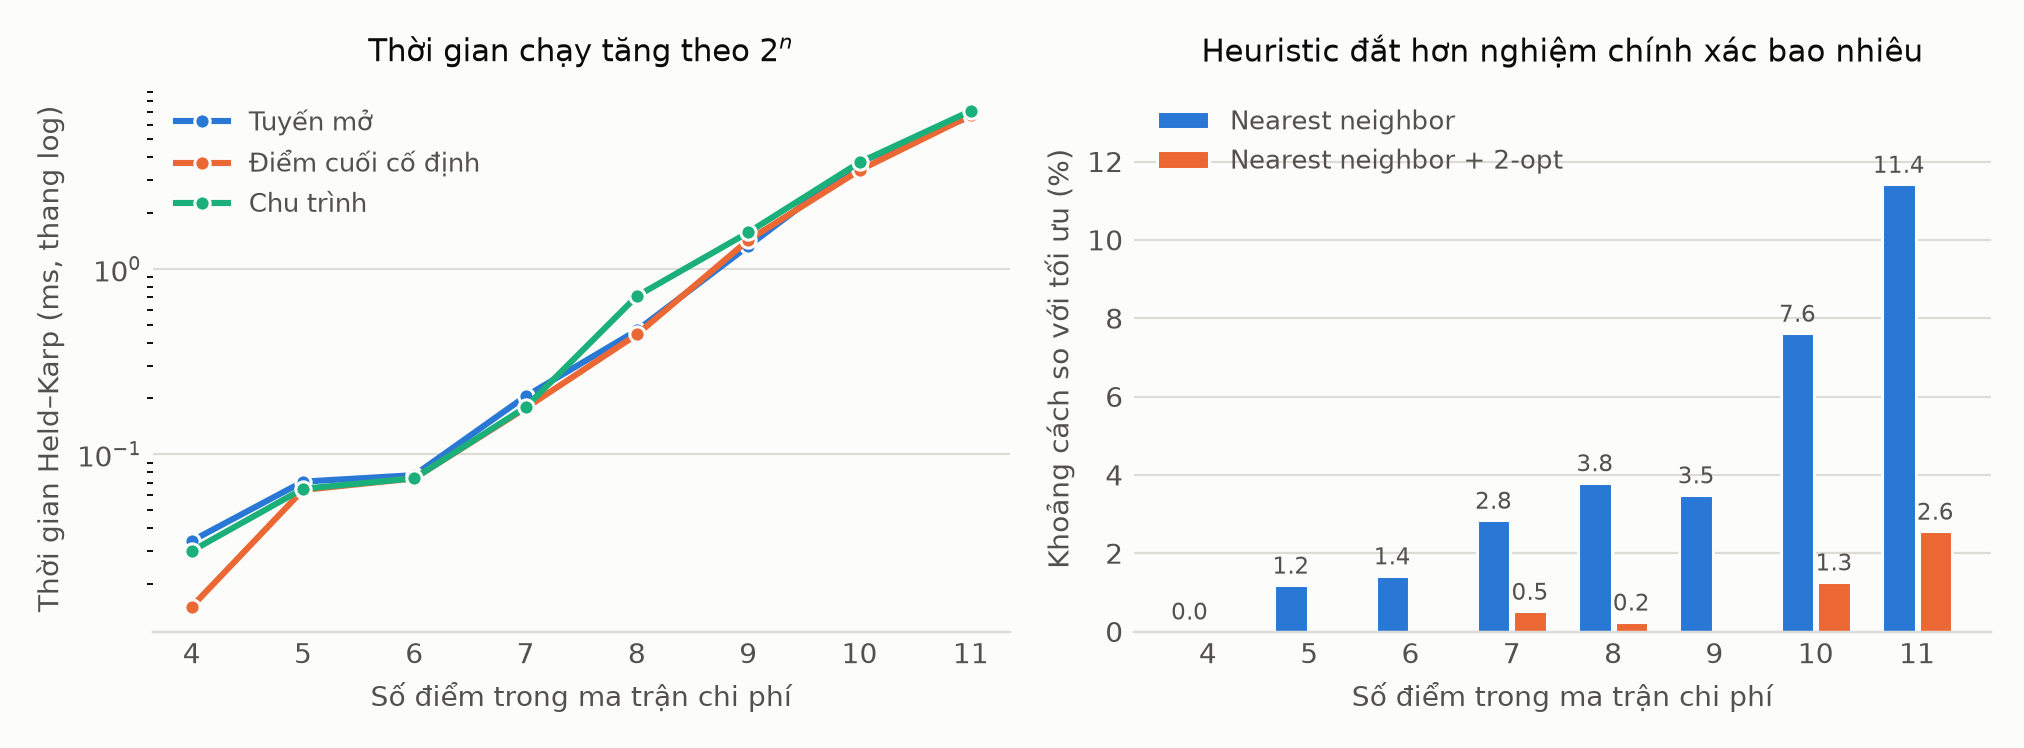
\includegraphics[width=\linewidth]{tsp-scaling.png}
\caption[Thời gian Held--Karp và khoảng cách chất lượng của heuristic]
{Trái: thời gian Held--Karp theo số điểm trên thang log, ba kiểu kết thúc.
Phải: khoảng cách trung bình so với nghiệm tối ưu của hai heuristic}
\label{fig:tsp-scaling}
\end{figure}

\begin{table}[H]
\centering
\small
\caption{Thời gian trung bình của ba thuật toán theo số điểm (kiểu chu trình)}
\label{tab:tsp-runtime}
\begin{tabular}{r r r r r r}
\toprule
\textbf{Điểm} & \textbf{Số trạng thái DP} & \textbf{Held--Karp} &
\textbf{NN} & \textbf{NN + 2-opt} & \textbf{Tỉ lệ tăng} \\
 & $(n-1)2^{\,n-1}$ & (ms) & (ms) & (ms) & Held--Karp \\
\midrule
4 & 24 & 0,030 & 0,008 & 0,019 & -- \\
5 & 64 & 0,065 & 0,009 & 0,039 & 2,17 \\
6 & 160 & 0,074 & 0,005 & 0,029 & 1,14 \\
7 & 384 & 0,179 & 0,007 & 0,041 & 2,42 \\
8 & 896 & 0,712 & 0,012 & 0,075 & 3,98 \\
9 & 2048 & 1,569 & 0,012 & 0,080 & 2,20 \\
10 & 4608 & 3,748 & 0,011 & 0,093 & 2,39 \\
11 & 10240 & 7,113 & 0,013 & 0,115 & 1,90 \\
\bottomrule
\end{tabular}
\end{table}

Cột cuối là tỉ số thời gian giữa hai kích thước liên tiếp. Trung bình nhân của các
tỉ số từ 7 đến 11 điểm là khoảng 2,4 lần cho mỗi điểm thêm vào, nằm quanh mức mà
công thức $O(n^2 2^n)$ dự đoán ở dải này. Hai giá trị nhỏ ở $n=5$ và $n=6$ là
nhiễu đo: ở mức vài chục micro giây, chi phí khởi tạo và dao động bộ đệm lấn át
phần tính toán, nên không nên đọc tỉ lệ tăng tại các kích thước nhỏ nhất.

Điều quan trọng về mặt kỹ thuật là mức tuyệt đối. Ở giới hạn thiết kế 10 điểm cần
ghé (11 điểm trong ma trận), Held--Karp vẫn chỉ tốn khoảng 7 ms, nhỏ hơn hai bậc
độ lớn so với bước lập ma trận chi phí. Nói cách khác, trong phạm vi mà giao diện
cho phép, tầng tổ hợp \textbf{không} phải nút cổ chai; chi phí thực tế nằm ở
Dijkstra trên graph lớn.

\begin{table}[H]
\centering
\caption{Thời gian lập ma trận chi phí bằng Dijkstra theo số điểm}
\label{tab:dijkstra-scaling}
\begin{tabular}{r r r}
\toprule
\textbf{Điểm} & \textbf{Số lần chạy Dijkstra} & \textbf{Thời gian (giây)} \\
\midrule
4 & 4 & 0,484 \\
5 & 5 & 0,806 \\
6 & 6 & 1,462 \\
7 & 7 & 1,618 \\
8 & 8 & 1,649 \\
9 & 9 & 1,860 \\
10 & 10 & 1,995 \\
11 & 11 & 2,218 \\
\bottomrule
\end{tabular}
\end{table}

Thời gian Dijkstra tăng gần tuyến tính theo số điểm chứ không theo giai thừa, vì
mỗi điểm chỉ thêm một lần chạy nguồn đơn nhiều đích. Tỉ lệ giữa hai tầng tại 11
điểm là khoảng $2{,}218$ giây so với $7{,}1$ ms, tức tầng đồ thị chiếm hơn 99,6\%
tổng thời gian tối ưu. Đây là lý do kiến trúc tách hai tầng và cache graph trong
phiên: muốn giảm thời gian chờ thì phải nhắm vào Dijkstra và việc nạp graph, không
phải vào Held--Karp.

\subsection{Diễn giải và giới hạn của phép đo}

Benchmark này cho phép kết luận ba điều trong phạm vi dữ liệu đã dùng: Held--Karp
khả thi về thời gian ở toàn bộ dải được hỗ trợ; nearest-neighbor có thể lệch hai
chữ số phần trăm khi tuyến bị ràng buộc điểm cuối; và 2-opt là một cải thiện rẻ
nhưng không phải một lời bảo đảm.

Giới hạn cần nói rõ: phép đo chỉ dùng một tập 11 địa điểm tại Hà Nội và các tập
con lồng nhau của nó, nên không phải một mẫu ngẫu nhiên của mọi cấu hình điểm. Với
tập điểm cụm chặt hoặc phân bố hình sao, thứ hạng heuristic có thể khác. Thời gian
đo trên một máy phát triển với Python 3.11 và không loại bỏ ảnh hưởng của tải hệ
thống; vì vậy tỉ lệ giữa các tầng đáng tin hơn giá trị tuyệt đối. Cuối cùng, phép
đo tách ma trận chi phí ra khỏi tầng tổ hợp một cách có chủ ý, nên các con số ở
Bảng~\ref{tab:tsp-runtime} không cộng lại thành thời gian người dùng cảm nhận;
Bảng~\ref{tab:dijkstra-scaling} mới là phần chiếm đa số thời gian đó.

\section{Thiết kế benchmark trò chơi}

Mỗi sân dùng 20 seed, ba bot người trốn và ba chiến thuật máy, tạo
$20\times3\times3=180$ ván/sân và 360 ván tổng cộng. Bộ luật cố định:
$b_r=b_h=160$ m, tiết lộ mỗi ba lượt, tối đa 18 lượt. Ba bot người trốn là:
\begin{itemize}
  \item \texttt{random}: chọn ngẫu nhiên trong các nút khả đạt;
  \item \texttt{nearest\_exit}: ưu tiên tiến về lối thoát gần nhất;
  \item \texttt{evasive}: ưu tiên tránh đội máy trong khi vẫn tìm lối thoát.
\end{itemize}

Bot và vị trí khởi đầu đều cố định theo seed. Vì không có người chơi thật, phép
đo chỉ đánh giá tương tác với ba hành vi lập trình sẵn. Không chiến thuật nào
trong hai phía được chứng minh tối ưu.

\section{Kết quả trên sân lưới mô phỏng}

\begin{table}[H]
\centering
\small
\caption{Benchmark sân lưới 81 nút; mỗi dòng gồm 20 ván}
\begin{tabular}{llrrrrrr}
\toprule
\textbf{Bot trốn} & \textbf{Máy} & \textbf{Thoát} & \textbf{Bắt} & \textbf{Hết lượt} &
\textbf{Lượt TB} & \textbf{ms/bước TB} & \textbf{ms max} \\
\midrule
Ngẫu nhiên & Dấu vết & 3 & 16 & 1 & 6,15 & 0,724 & 3,470 \\
Ngẫu nhiên & Tìm kiếm & 2 & 18 & 0 & 4,45 & 0,882 & 3,523 \\
Ngẫu nhiên & Phối hợp & 1 & 19 & 0 & 4,80 & 3,973 & 14,897 \\
Gần lối thoát & Dấu vết & 18 & 2 & 0 & 3,15 & 0,628 & 2,806 \\
Gần lối thoát & Tìm kiếm & 19 & 1 & 0 & 3,20 & 0,870 & 2,828 \\
Gần lối thoát & Phối hợp & 13 & 7 & 0 & 3,20 & 2,972 & 10,620 \\
Né tránh & Dấu vết & 19 & 1 & 0 & 3,90 & 0,589 & 3,147 \\
Né tránh & Tìm kiếm & 20 & 0 & 0 & 3,70 & 1,119 & 3,345 \\
Né tránh & Phối hợp & 19 & 1 & 0 & 4,50 & 3,304 & 11,581 \\
\bottomrule
\end{tabular}
\end{table}

Trên bot ngẫu nhiên, phối hợp bắt 19/20 ván, cao hơn dấu vết 16/20. Trên bot đi
thẳng tới lối thoát, phối hợp bắt 7/20, trong khi hai chiến thuật còn lại chỉ bắt
2/20 và 1/20. Đây là bằng chứng cấu hình cụ thể cho lợi ích của thành phần chặn
lối thoát. Tuy nhiên bot né tránh vẫn thoát 19/20 trước phối hợp. Tổng trên 60
ván/chiến thuật, phối hợp bắt 27 ván, còn dấu vết và tìm kiếm cùng bắt 19 ván.

Đổi lại, phối hợp tốn 2,972--3,973 ms/bước trung bình, cao hơn các chính sách đơn
dưới 1,2 ms ở phần lớn cấu hình. Mức này vẫn phù hợp tương tác, nhưng phản ánh chi
phí xét tổ hợp ứng viên giữa hai đội.

\section{Kết quả trên sân OSM cục bộ}

\begin{table}[H]
\centering
\small
\caption{Benchmark sân OSM 358 nút; mỗi dòng gồm 20 ván}
\begin{tabular}{llrrrrrr}
\toprule
\textbf{Bot trốn} & \textbf{Máy} & \textbf{Thoát} & \textbf{Bắt} & \textbf{Hết lượt} &
\textbf{Lượt TB} & \textbf{ms/bước TB} & \textbf{ms max} \\
\midrule
Ngẫu nhiên & Dấu vết & 0 & 20 & 0 & 8,25 & 2,026 & 11,804 \\
Ngẫu nhiên & Tìm kiếm & 0 & 20 & 0 & 7,95 & 2,580 & 10,702 \\
Ngẫu nhiên & Phối hợp & 0 & 19 & 1 & 9,30 & 5,241 & 18,427 \\
Gần lối thoát & Dấu vết & 16 & 4 & 0 & 6,30 & 2,137 & 11,864 \\
Gần lối thoát & Tìm kiếm & 15 & 5 & 0 & 5,95 & 2,297 & 8,666 \\
Gần lối thoát & Phối hợp & 16 & 4 & 0 & 6,15 & 4,255 & 12,369 \\
Né tránh & Dấu vết & 15 & 1 & 4 & 9,65 & 1,816 & 8,055 \\
Né tránh & Tìm kiếm & 15 & 1 & 4 & 9,90 & 2,273 & 8,620 \\
Né tránh & Phối hợp & 13 & 2 & 5 & 9,85 & 3,716 & 11,151 \\
\bottomrule
\end{tabular}
\end{table}

Trên sân OSM, cả ba chiến thuật bắt toàn bộ hoặc gần toàn bộ bot ngẫu nhiên.
Với bot gần lối thoát, số ván bắt chỉ từ 4 đến 5; với bot né tránh, chỉ từ 1 đến
2, còn 4--5 ván kết thúc do hết lượt. Tổng số bắt trên 60 ván lần lượt là 25,
26 và 25 cho dấu vết, tìm kiếm và phối hợp. Vì vậy benchmark này bác bỏ cách diễn
giải đơn giản rằng phối hợp luôn mạnh nhất.

Sự khác biệt giữa sân lưới và OSM có thể do topology, vị trí lối thoát, đường cụt
và shortlist ứng viên, nhưng benchmark hiện tại chưa cô lập nguyên nhân. Đây là
giả thuyết cần thí nghiệm ablation, không phải kết luận đã kiểm chứng.

\begin{figure}[H]
\centering
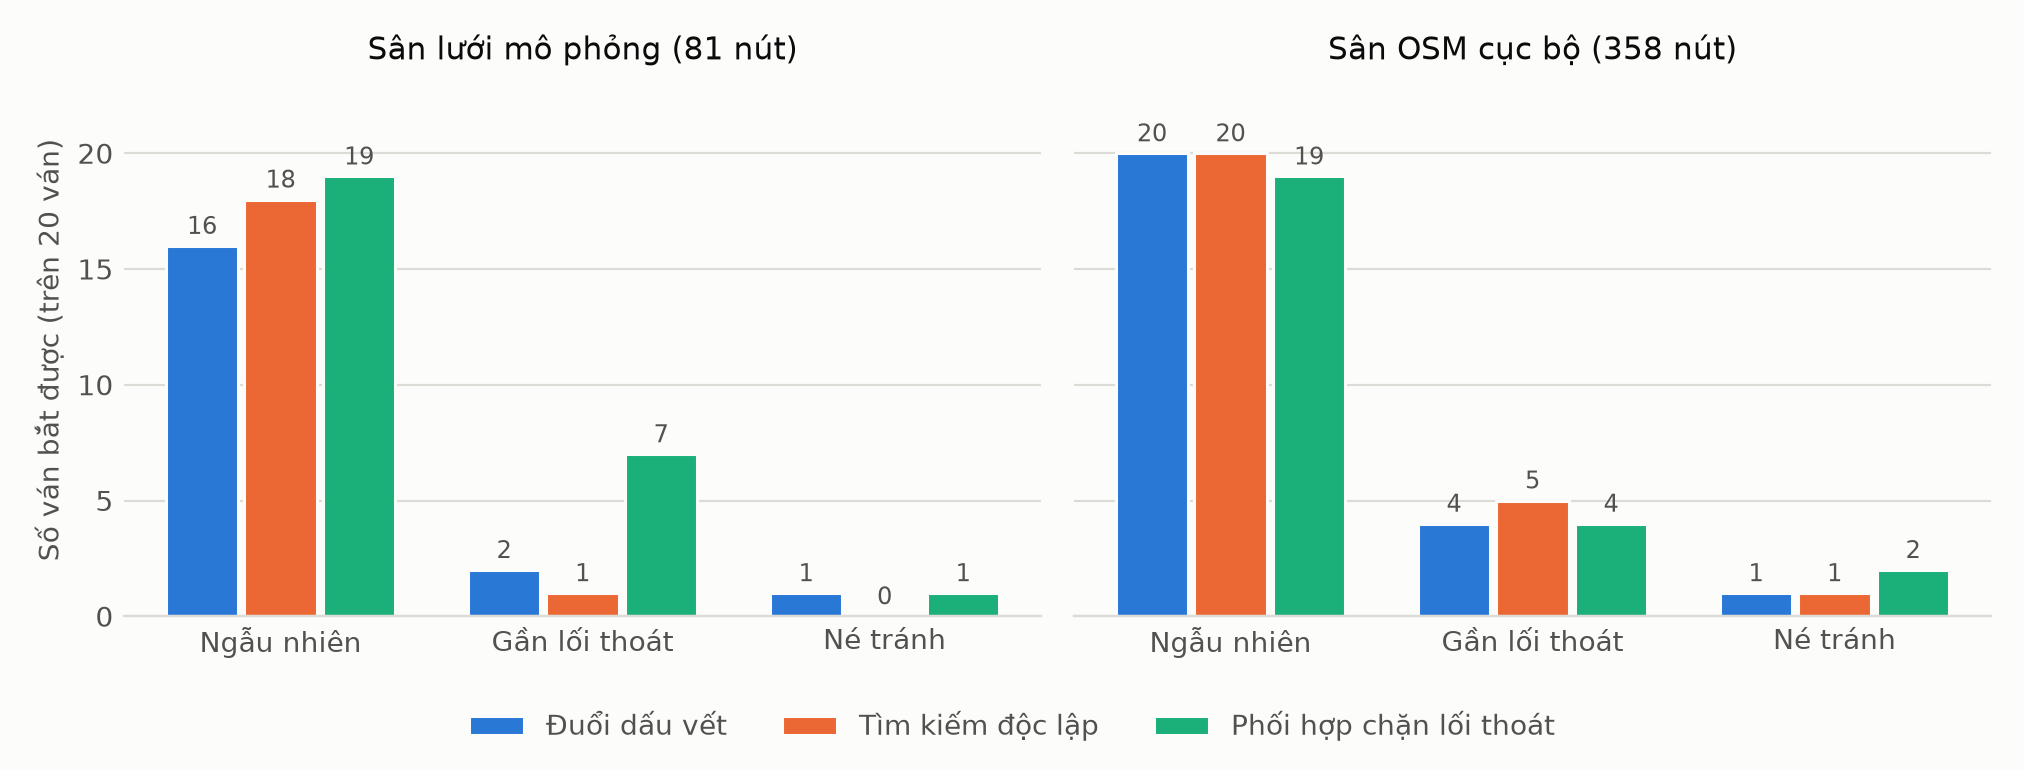
\includegraphics[width=\linewidth]{benchmark-capture.png}
\caption[Số ván bắt được theo chiến thuật máy và bot người trốn]
{Số ván bắt được trên mỗi cấu hình 20 ván, đối chiếu hai sân. Thứ hạng ba chiến
thuật đảo khi đổi sân và đổi bot người trốn}
\label{fig:benchmark-capture}
\end{figure}

Hình~\ref{fig:benchmark-capture} đặt hai sân cạnh nhau để thấy rõ điều mà hai bảng
số rời rạc dễ che: lợi thế của chiến thuật phối hợp chỉ xuất hiện ở sân lưới và
chỉ với hai trong ba bot, còn trên sân OSM ba cột gần như bằng nhau ở mọi nhóm.
Nếu một chiến thuật thực sự trội, các cột xanh lục phải cao hơn ở cả sáu nhóm;
dữ liệu không cho thấy điều đó.

\section{Đánh giá giao diện và tích hợp}

AppTest kiểm tra mở mặc định ở Lộ trình, deep link tới Trốn tìm, chuyển qua lại
và giữ tiêu chí/kiểu điểm cuối/click bản đồ. Các kịch bản game đi đến ba kết cục
\texttt{escaped}, \texttt{caught}, \texttt{timeout}. Playwright được dùng để
kiểm tra trình duyệt thật: chọn Hồ Hoàn Kiếm tới Nhà hát Lớn, tối ưu được tuyến
1,36 km với thời gian hiển thị 1,4 phút; chuyển sang trò chơi rồi quay lại vẫn
giữ nguyên kết quả.

\begin{figure}[H]
\centering
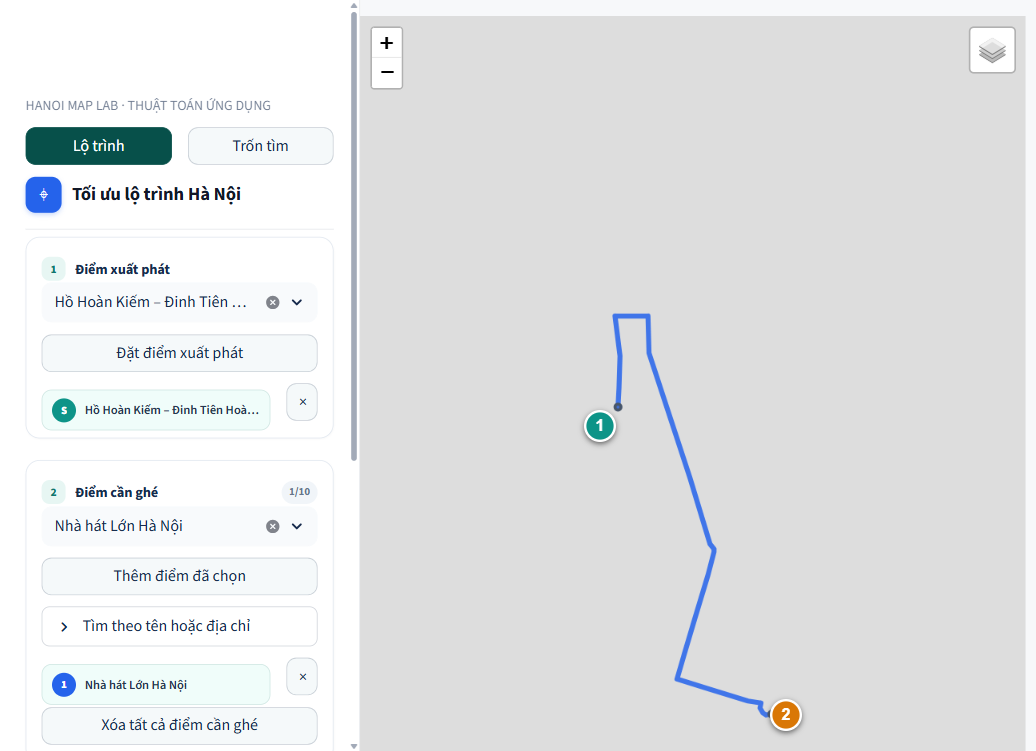
\includegraphics[width=0.92\linewidth]{route-result.png}
\caption{Tuyến thực được vẽ sau khi tối ưu trong giao diện tích hợp}
\label{fig:route-result}
\end{figure}

Trong ảnh kiểm tra, tile nền màu xám do sự cố phân giải/chính sách mạng của máy
thử nghiệm, nhưng polyline và chỉ số thuật toán vẫn hiển thị. Điều này minh họa
việc tile nền và graph định tuyến là hai thành phần độc lập.

\section{Các mối đe dọa tới tính hợp lệ}

\textbf{Tính hợp lệ nội tại:} benchmark dùng cùng seed giữa các chiến thuật, nhưng
không thực hiện kiểm định thống kê hoặc hoán đổi ngẫu nhiên thứ tự chạy. Thời gian
có thể bị ảnh hưởng bởi warm cache và tải hệ thống.

\textbf{Tính hợp lệ cấu trúc:} tỉ lệ bắt/thoát đo hiệu quả trong luật trò chơi đã
định nghĩa, không đo chất lượng chiến thuật trong pursuit--evasion liên tục. Hàm
coverage là proxy khoảng cách, không phải xác suất bắt.

\textbf{Tính hợp lệ ngoại suy:} chỉ có hai sân, ba bot và 20 seed. Sân OSM là
phần graph cục bộ đã điều chỉnh hai chiều. Không thể suy ra hiệu quả trên toàn Hà
Nội, người chơi thật hoặc điều kiện giao thông thực tế.

\textbf{Tính đúng dữ liệu:} trọng số thời gian là ước tính tĩnh. Kết quả 29,93
phút không phải dự báo thời gian thực và không nên dùng như chỉ dẫn giao thông.

\chapter{Minh Chứng Sản Phẩm Và Kịch Bản Demo}

\section{Khởi chạy ứng dụng}

Từ PowerShell tại thư mục dự án, dùng môi trường Python 3.11 đã cài dependency:

\begin{lstlisting}[language=bash,caption={Lệnh khởi chạy ứng dụng}]
.\.venv\Scripts\python.exe -m streamlit run app.py --server.port 8502
\end{lstlisting}

Mở \url{http://localhost:8502}. Mặc định ứng dụng vào chế độ Lộ trình. Query
\texttt{?mode=chase} mở trực tiếp chế độ Trốn tìm. Graph định tuyến lớn cần thời
gian nạp lần đầu; các lần tương tác sau dùng cache.

\section{Kịch bản demo chế độ Lộ trình}

Kịch bản đề xuất dài khoảng ba phút:
\begin{enumerate}
  \item Chọn Đại học Phenikaa làm điểm xuất phát; thêm Mỹ Đình, Cầu Giấy, Hồ Tây
  và Hồ Hoàn Kiếm làm điểm cần ghé.
  \item Chọn mục tiêu \textit{Quãng đường}, điểm cuối tự động và bấm tối ưu.
  Giải thích pipeline Dijkstra $\rightarrow$ ma trận chi phí $\rightarrow$
  Held--Karp $\rightarrow$ khôi phục tuyến.
  \item Đọc thứ tự ghé, tổng km, thời gian ước tính và thời gian từng thuật toán.
  \item Chuyển mục tiêu sang \textit{Thời gian di chuyển}; chỉ ra rằng tuyến có
  thể dài hơn nhưng thời gian ước tính thấp hơn.
  \item Chọn điểm cuối cố định hoặc quay về điểm đầu để minh họa ba biến thể.
\end{enumerate}

Khi trình bày, cần nói rõ Held--Karp tối ưu chính xác trên ma trận chi phí của các
điểm đã chọn, không phải giải mọi biến thể VRP. Tile nền không tham gia phép tính.

\section{Kịch bản demo chế độ Trốn tìm}

Nhấn \textit{Trốn tìm}, chọn sân phố Hà Nội, chiến thuật \textit{Phối hợp chặn
lối thoát}, seed 7 và giữ bộ luật mặc định. Bắt đầu ván mới; giải thích màu xanh
lá là người chơi, đỏ là đội máy, xanh dương là lối thoát, các chấm xanh nhạt là
điểm đến hợp lệ.

\begin{figure}[H]
\centering
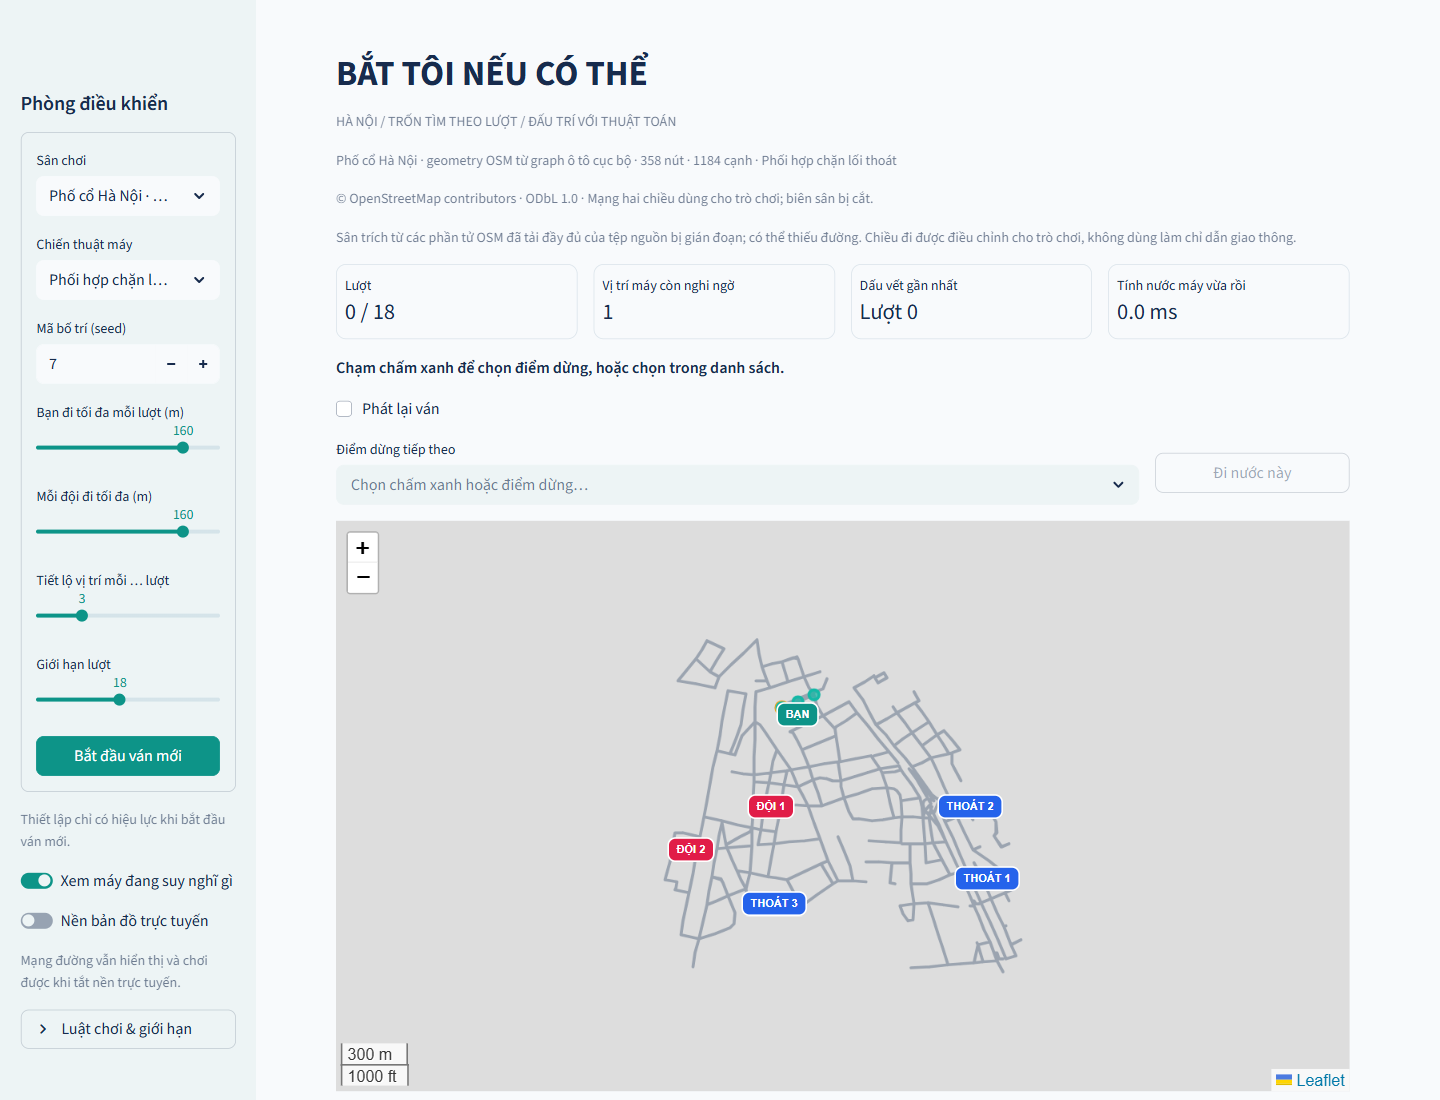
\includegraphics[width=0.95\linewidth]{chase-map.png}
\caption[Phòng điều khiển và trạng thái đầu ván]
{Phòng điều khiển cùng trạng thái đầu ván trên sân phố cổ Hà Nội: bộ luật đang
dùng nằm ở cột trái, bốn chỉ số trạng thái nằm trên bản đồ. Ở lượt 0, vị trí
người trốn vừa được tiết lộ nên ``Vị trí máy còn nghi ngờ'' bằng 1}
\label{fig:chase-control}
\end{figure}

Bảng điều khiển ở Hình~\ref{fig:chase-control} là nơi nên dừng lại khi trình bày:
mọi tham số của bộ luật đều hiện rõ, nên người nghe kiểm chứng được rằng kết quả
ván chơi phụ thuộc vào cấu hình chứ không phải một hộp đen. Lưu ý thiết lập chỉ có
hiệu lực khi bắt đầu ván mới, vì vậy cần chốt thông số trước khi bấm nút.

\begin{figure}[H]
\centering
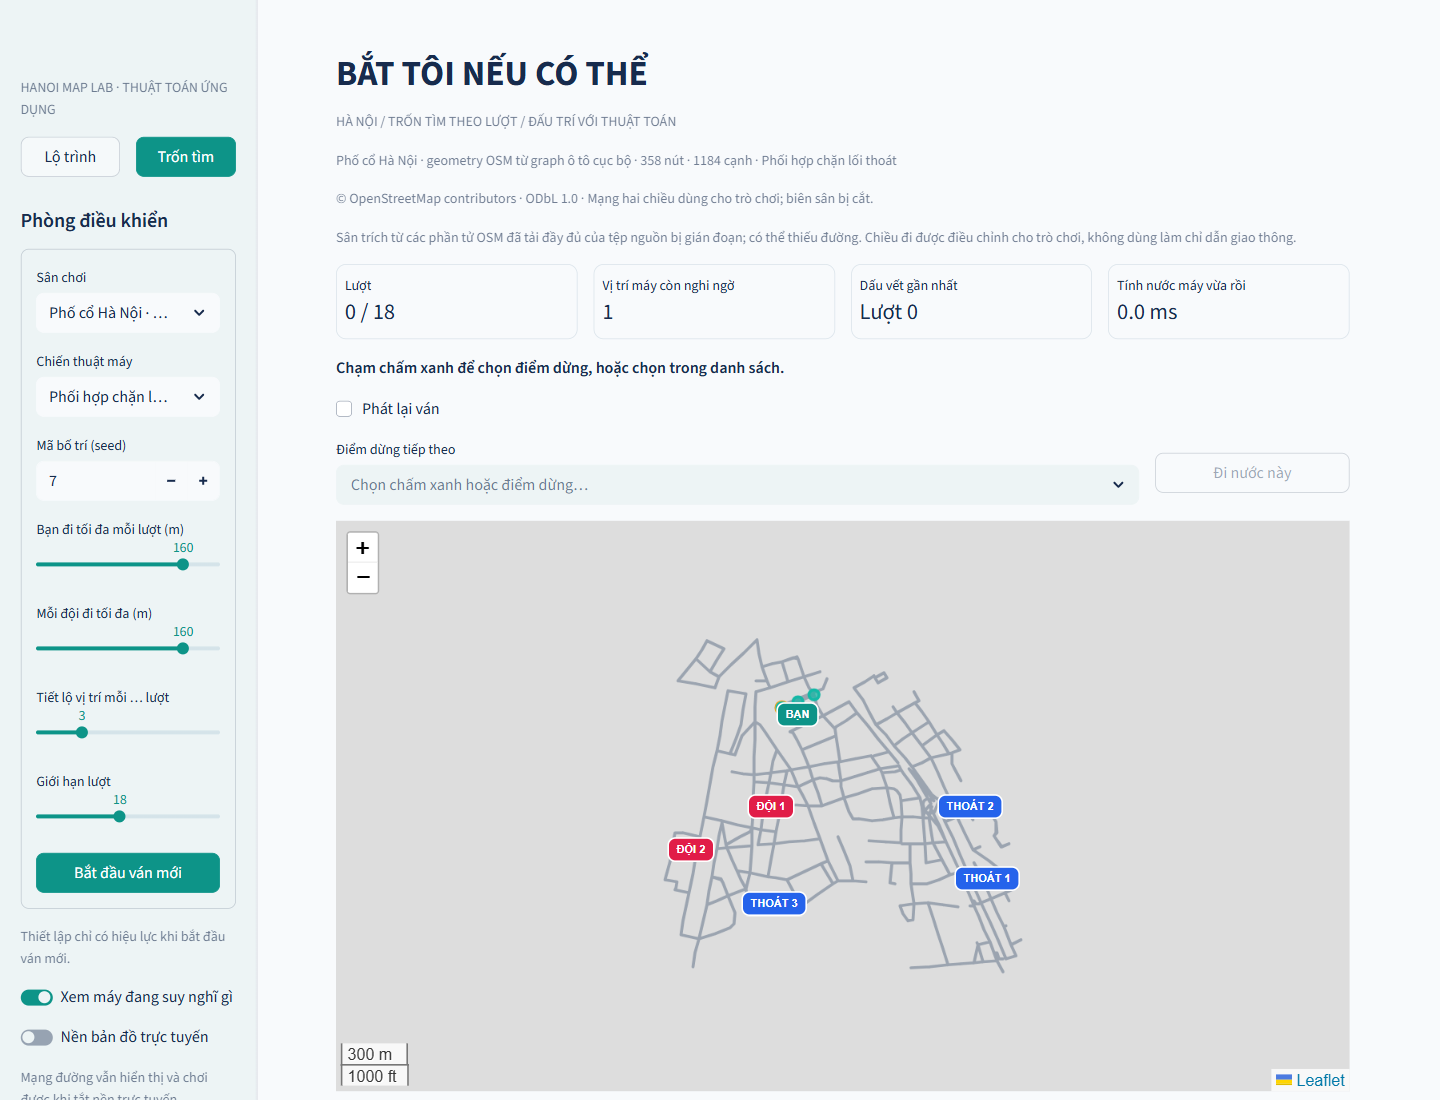
\includegraphics[width=0.92\linewidth]{chase-ui.png}
\caption{Giao diện trò chơi trên graph phố Hà Nội cục bộ}
\label{fig:chase-ui}
\end{figure}

Chơi ít nhất ba lượt để xuất hiện một lần tiết lộ. Trước lượt tiết lộ, chỉ ra số
``Vị trí máy còn nghi ngờ'' tăng theo reachability; ở lượt tiết lộ, tập này co về
một nút. Bật tùy chọn xem giải thích để đọc mục tiêu mà máy chọn. Sau đó bật phát
lại, kéo slider qua các lượt và tải JSON lịch sử.

\section{Thông điệp thuật toán cần nhấn mạnh}

\begin{table}[H]
\centering
\caption{Thông điệp bảo vệ đồ án và bằng chứng tương ứng}
\begin{tabularx}{\linewidth}{Y Y}
\toprule
\textbf{Thông điệp} & \textbf{Bằng chứng có thể trình diễn} \\
\midrule
Dijkstra giải đường đi giữa cặp điểm trên graph có hướng & Polyline chi tiết,
ma trận chi phí và test oracle ngẫu nhiên \\
Held--Karp là tối ưu chính xác trong miền nhỏ & So sánh với vét cạn ở test; thời
gian dưới 0,2 ms trong smoke test 5 điểm \\
Heuristic không có bảo đảm tối ưu & Bảng benchmark cho thấy thứ hạng thay đổi
theo bot và sân \\
Máy không biết vị trí ẩn & API \texttt{Observation} và test hai trạng thái ẩn có
cùng quan sát \\
Giao diện không thay thế kiểm thử & 112 unit/integration test cùng kiểm tra trình
duyệt thật \\
\bottomrule
\end{tabularx}
\end{table}

\section{Tình huống lỗi và phương án phục hồi}

Nếu tile nền không tải, chuyển layer vệ tinh nếu khả dụng hoặc tiếp tục demo
graph/marker; không cần tải lại dữ liệu định tuyến. Nếu graph lớn chưa nạp được,
chuyển sang Trốn tìm vì sân nhỏ độc lập, sau đó kiểm tra Git LFS. Nếu thao tác
game bị chọn sai nút, dùng dropdown điểm đến thay cho click. Nếu demo cần tái lập,
giữ nguyên seed và thông số trước khi bấm bắt đầu ván mới.

\begin{notebox}[title={Giới hạn cần nói công khai khi bảo vệ}]
Sân OSM của trò chơi chỉ là một phần mạng đường và đã chuyển hai chiều; trọng số
thời gian của định tuyến là ước tính tĩnh; benchmark dùng bot viết sẵn; chiến
thuật phối hợp là heuristic. Các giới hạn này không làm mất giá trị đồ án, nhưng
quyết định phạm vi mà kết quả có thể hỗ trợ.
\end{notebox}

\chapter{Kết Luận Và Hướng Phát Triển}

\section{Kết quả đạt được}

Đồ án đã hoàn thành một ứng dụng thuật toán đồ thị gồm hai chế độ tích hợp. Phần
định tuyến xử lý graph ô tô Hà Nội quy mô 350.930 nút và 864.982 cạnh, hỗ trợ
tối đa 10 điểm ghé, hai hàm mục tiêu và ba kiểu kết thúc. Phần thuật toán tách
rõ Dijkstra cho đường đi giữa cặp điểm, Held--Karp cho thứ tự ghé chính xác và
hai heuristic để đối chiếu. Benchmark 24 cấu hình xác nhận cả hai mặt của cách
tách này: Held--Karp giữ thời gian dưới 7,2 ms ở giới hạn 10 điểm ghé, còn
heuristic đổi bảo đảm tối ưu lấy tốc độ với cái giá đo được là tới 19,53\% chi
phí dư thừa khi tuyến bị ràng buộc điểm cuối.

Phần trò chơi mở rộng bài toán từ tối ưu tĩnh sang ra quyết định tuần tự dưới
thông tin không đầy đủ. Tập niềm tin, chu kỳ tiết lộ và ranh giới
\texttt{Observation} làm rõ máy biết gì ở mỗi lượt. Ba chiến thuật có mức phức
tạp và hành vi khác nhau, được so sánh trên 360 ván tái lập.

Bộ 112 test đều đạt trong lần chạy ngày 24/10/2026. Smoke test và kiểm tra trình
duyệt chứng minh pipeline hoạt động trên graph thật và trạng thái được giữ khi
chuyển chế độ. Sản phẩm có replay, log JSON và thông báo giới hạn dữ liệu để hỗ
trợ trình diễn và kiểm tra.

\section{Bài học thuật toán}

Thứ nhất, một bài toán ứng dụng thường cần ghép nhiều tầng tối ưu. Dijkstra đúng
cho từng đoạn chưa quyết định được thứ tự ghé; Held--Karp giải tầng tổ hợp sau khi
ma trận chi phí được tạo. Thứ hai, thuật toán chính xác và heuristic có vai trò
khác nhau: chính xác cho bảo đảm trong miền nhỏ, heuristic đổi bảo đảm lấy tốc độ
hoặc hành vi thực dụng. Thứ ba, trong hệ thống thông tin ẩn, định nghĩa giao diện
quan sát quan trọng không kém hàm đánh giá; nếu policy đọc được trạng thái thật,
mọi kết quả chiến thuật trở nên vô nghĩa.

Cuối cùng, kiểm thử cần bám vào giả định và bất biến. Kiểm tra một nút bấm hoạt
động không chứng minh thuật toán đúng; ngược lại, unit test không chứng minh giao
diện sử dụng được. Đồ án kết hợp oracle, test biên, AppTest, smoke test và trình
duyệt thật để giảm khoảng cách này.

\section{Hạn chế}

\begin{itemize}
  \item Thời gian di chuyển là tĩnh, chưa có dữ liệu ùn tắc theo thời điểm.
  \item Benchmark tầng thứ tự ghé chỉ dùng một tập 11 địa điểm và các tập con lồng
  nhau, chưa lấy mẫu ngẫu nhiên trên nhiều dạng phân bố điểm.
  \item Held--Karp tăng theo $2^n$, nên giới hạn hiện tại là 10 điểm ghé.
  \item Hệ thống chưa giải VRP nhiều xe, time window, capacity hoặc điểm động
  \cite{toth2014}.
  \item Graph trò chơi OSM không đầy đủ và được điều chỉnh hai chiều.
  \item Bắt chỉ xét vị trí nút sau bước đi; chưa xét hai tác nhân giao nhau giữa cạnh.
  \item Tập niềm tin không mang xác suất; hệ số 0,35 và shortlist 8 ứng viên chưa
  được hiệu chỉnh độc lập.
  \item Benchmark chỉ có ba bot, hai sân và 20 seed; chưa có người chơi thật hoặc
  kiểm định thống kê.
  \item Lớp tile trực tuyến phụ thuộc DNS và chính sách nhà cung cấp, dù thuật
  toán cục bộ không phụ thuộc lớp nền.
\end{itemize}

\section{Hướng phát triển có thứ tự ưu tiên}

\textbf{Ưu tiên 1 -- củng cố đánh giá.} Mở rộng seed và topology, thêm baseline
ngẫu nhiên, chạy ablation hệ số lối thoát/shortlist/chu kỳ tiết lộ, báo khoảng tin
cậy và thu thập một tập ván người chơi. Tiêu chí tiếp tục là kết quả lặp lại qua
nhiều sân; nếu ưu thế chỉ xuất hiện trên lưới, cần thu hẹp claim thay vì đổi tên
chiến thuật.

\textbf{Ưu tiên 2 -- xác suất hóa niềm tin.} Thay tập $B_t$ bằng phân phối
$p_t(v)$ với mô hình chuyển của người trốn, sau đó đánh giá expected capture hoặc
information gain. Cần có positive control: khi mô hình chuyển đúng với bot sinh
dữ liệu, phương pháp xác suất phải cải thiện so với uniform belief; nếu không,
cơ chế chưa được hỗ trợ.

\textbf{Ưu tiên 3 -- lập kế hoạch nhiều bước.} So sánh heuristic một bước với
beam search hoặc Monte Carlo tree search \cite{browne2012} trên sân nhỏ. Trước khi mở rộng, cần đo
trade-off giữa tỉ lệ bắt và độ trễ; không gọi là tối ưu nếu chưa có chứng minh
hoặc oracle kích thước nhỏ.

\textbf{Ưu tiên 4 -- định tuyến động và bền vững.} Nếu có dữ liệu thời gian theo
cạnh $c_{ij}(t)$, mô hình phải kiểm tra thuộc tính FIFO và chạy thuật toán phù
hợp; không dùng một hệ số ``giờ cao điểm'' toàn cục rồi gọi đó là time-dependent
routing. Một hướng gần hơn là cho phép chặn một số cạnh và đo độ tăng chi phí,
tạo kịch bản ``phá đường--cứu tuyến'' có đối chứng rõ ràng.

\section{Kết luận chung}

Hệ thống cho thấy một đề tài tối ưu lộ trình truyền thống có thể phát triển thành
một phòng thí nghiệm thuật toán đồ thị có tính tương tác mà vẫn giữ được phần lõi
ban đầu. Giá trị chính không nằm ở tuyên bố một chiến thuật luôn tốt nhất, mà ở
việc mô hình hóa rõ, triển khai có ranh giới thông tin, so sánh đúng mức và cung
cấp bằng chứng tái lập. Đây là nền tảng phù hợp để tiếp tục nghiên cứu các bài
toán định tuyến và pursuit--evasion phức tạp hơn.

\appendix
\chapter{Phụ Lục Tái Lập}

\section{Cài đặt trên Windows 11}

\begin{lstlisting}[language=bash,caption={Tạo môi trường và cài dependency}]
py -3.11 -m venv .venv
.\.venv\Scripts\python.exe -m pip install -r requirements.txt
git lfs pull
\end{lstlisting}

Hai graph lớn được quản lý bằng Git LFS. Nếu tệp chỉ có vài dòng pointer, cần
cài Git LFS và chạy lại \texttt{git lfs pull} trước khi đánh giá định tuyến.

\section{Lệnh kiểm thử và benchmark}
\label{sec:lenh-tai-lap}

\begin{lstlisting}[language=bash,caption={Các lệnh tái lập kết quả chính}]
.\.venv\Scripts\python.exe -m unittest discover -s tests -q
.\.venv\Scripts\python.exe scripts\smoke_offline.py
.\.venv\Scripts\python.exe scripts\benchmark_chase.py `
  --source demo --seeds 20 --output output\chase\benchmark-demo.json
.\.venv\Scripts\python.exe scripts\benchmark_chase.py `
  --source osm --seeds 20 --output output\chase\benchmark-osm.json
.\.venv\Scripts\python.exe scripts\benchmark_tsp.py --weight length
.\.venv\Scripts\python.exe scripts\benchmark_tsp.py --weight travel_time `
  --output output\routing\benchmark-tsp-time.json
\end{lstlisting}

PowerShell dùng dấu backtick để nối dòng. Trên shell khác, thay bằng ký tự nối
dòng tương ứng hoặc viết mỗi lệnh trên một dòng.

\section{Cấu trúc mã nguồn và quy mô}

\begin{lstlisting}[language=bash,caption={Cây thư mục dự án (bỏ qua tệp sinh ra)}]
Hanoi_map_optimizer/
|-- app.py                      # diem vao Streamlit, chuyen che do
|-- chase_app.py                # shortcut mo thang che do Tron tim
|-- data/
|   |-- popular_locations.py    # 13 dia diem mau da kiem tra toa do
|   |-- hanoi_urban_drive.pkl   # graph dinh tuyen (Git LFS)
|   |-- hanoi_urban_drive.graphml
|   `-- hanoi_urban_drive.meta.json
|-- src/
|   |-- shortest_path.py        # Dijkstra + ma tran chi phi
|   |-- tsp.py                  # Held-Karp cho ba kieu ket thuc
|   |-- heuristics.py           # nearest-neighbor, 2-opt
|   |-- route_optimizer.py      # dieu phoi pipeline dinh tuyen
|   |-- map_service.py          # nap/cache graph, kiem tra metadata
|   |-- chase.py                # luat, Observation, ba chien thuat
|   |-- chase_maps.py           # san luoi, san OSM, sinh kich ban
|   |-- chase_ui.py             # dieu khien van, replay, xuat JSON
|   |-- visualization.py        # ve ban do Folium
|   |-- geocoding.py            # tim dia diem theo ten
|   |-- utils.py, constants.py  # kieu du lieu chung, hang so
|-- tests/                      # 112 ca kiem thu tren 11 tep
|-- scripts/
|   |-- smoke_offline.py        # smoke test tren graph dong goi
|   |-- benchmark_tsp.py        # benchmark tang thu tu ghe
|   |-- benchmark_chase.py      # benchmark 360 van tro choi
|   |-- make_report_figures.py  # sinh hinh bieu do cho bao cao
|   `-- preload_hanoi*.py       # chuan bi du lieu OSM
|-- output/                     # ket qua benchmark dang JSON
`-- report/                     # bao cao LaTeX nay
\end{lstlisting}

\begin{table}[H]
\centering
\caption{Quy mô mã nguồn theo nhóm tệp}
\label{tab:quy-mo-ma}
\begin{tabular}{l r r}
\toprule
\textbf{Nhóm} & \textbf{Số tệp Python} & \textbf{Số dòng} \\
\midrule
Giao diện (\texttt{app.py}, \texttt{chase\_app.py}) & 2 & 745 \\
Thuật toán và dịch vụ (\texttt{src/}) & 13 & 1.425 \\
Kiểm thử (\texttt{tests/}) & 12 & 1.344 \\
Script dữ liệu và benchmark (\texttt{scripts/}) & 9 & 891 \\
Dữ liệu điểm mẫu (\texttt{data/}) & 2 & 19 \\
\midrule
\textbf{Tổng} & \textbf{38} & \textbf{4.424} \\
\bottomrule
\end{tabular}
\end{table}

Tỉ lệ giữa mã kiểm thử và mã thuật toán xấp xỉ 0,94:1. Con số này không phải mục
tiêu tự thân, nhưng cho thấy phần kiểm chứng được đầu tư tương đương phần triển
khai.

\section{Kết quả chạy bộ kiểm thử}

\begin{lstlisting}[language=bash,caption={Kết xuất rút gọn của lần chạy ngày 24/10/2026}]
> .\.venv\Scripts\python.exe -m unittest discover -s tests -q

[... cac dong log cua test duong loi, vi du: ]
_pickle.UnpicklingError: invalid load key, 'n'.
2026-10-24 09:07:56.798 No runtime found, using MemoryCacheStorageManager
----------------------------------------------------------------------
Ran 112 tests in 18.431s

OK
\end{lstlisting}

Dòng \texttt{UnpicklingError} ở trên đến từ ca kiểm thử cố ý nạp một tệp Pickle
hỏng để xác nhận hệ thống báo lỗi thân thiện thay vì sập. Traceback được in ra là
dữ liệu của test, không phải test thất bại; kết luận nằm ở hai dòng cuối.

\section{Lược đồ tệp kết quả benchmark}

Mọi số liệu ở Chương~5 đều được lưu dưới dạng JSON để có thể kiểm tra lại mà không
cần chạy lại. Hai lược đồ như sau.

\begin{lstlisting}[language=bash,caption={Lược đồ \texttt{output/routing/benchmark-tsp.json}}]
{
  "weight": "length",            # muc tieu toi uu
  "repeats": 5,                  # so lan lap moi cau hinh
  "graph_nodes": 350930,
  "graph_edges": 864982,
  "max_snap_distance_m": 263.22,
  "locations": [ ... ],          # ten 11 dia diem theo thu tu chi so
  "dijkstra_scaling": [ {"points": 4, "dijkstra_seconds": 0.484}, ... ],
  "results": [
    {
      "points": 11, "destinations": 10, "route_mode": "fixed_end",
      "states": 10240,           # (n-1) * 2^(n-1)
      "exact_order": [0, 9, 8, ...],
      "unit": "km",
      "exact_cost": 55.512,      # nghiem Held-Karp
      "nn_cost": 66.351, "nn_gap_percent": 19.53, "nn_mean_ms": 0.012,
      "two_opt_cost": 57.718, "two_opt_gap_percent": 3.97,
      "held_karp_mean_ms": 6.736, "held_karp_min_ms": 6.2
    }
  ],
  "status": "OK"
}
\end{lstlisting}

\begin{lstlisting}[language=bash,caption={Lược đồ \texttt{output/chase/benchmark-*.json}}]
{
  "source": "demo",              # "demo" (san luoi) hoac "osm"
  "nodes": 81, "edges": 288,
  "rules": {"runner_budget": 160, "hunter_budget": 160,
            "reveal_every": 3, "max_turns": 18},
  "seeds": [0, 1, ..., 19],
  "results": [
    {
      "runner": "nearest_exit",  # random | nearest_exit | evasive
      "hunter": "contain",       # trail | search | contain
      "games": 20,
      "escaped": 13, "caught": 7, "timeout": 0,
      "mean_turns": 3.2,
      "mean_step_ms": 2.972, "max_step_ms": 10.62
    }
  ]
}
\end{lstlisting}

Bất biến kiểm tra được trên mỗi dòng kết quả là
\texttt{escaped + caught + timeout = games}. Nếu tổng không khớp, hoặc benchmark
dừng giữa chừng, hoặc một kết cục chưa được phân loại.

\section{Sinh lại hình vẽ của báo cáo}

Hai hình biểu đồ được sinh từ chính các tệp JSON ở trên, không vẽ tay. Script cần
\texttt{matplotlib}, thư viện này cố ý không nằm trong \texttt{requirements.txt}
của ứng dụng vì chỉ phục vụ việc soạn báo cáo.

\begin{lstlisting}[language=bash,caption={Sinh lại hình và biên dịch báo cáo}]
python -m pip install matplotlib
python scripts\make_report_figures.py
cd report
latexmk -xelatex main.tex
\end{lstlisting}

Bảng màu của biểu đồ dùng ba màu phân loại đã được kiểm định về độ tương phản và
khả năng phân biệt với người mù màu; mỗi cột đều có nhãn số trực tiếp để không
phụ thuộc hoàn toàn vào màu sắc khi in đen trắng.

\section{Ma trận trường hợp kết thúc trò chơi}

\begin{table}[H]
\centering
\caption{Thứ tự ưu tiên các điều kiện trong một lượt}
\begin{tabularx}{\linewidth}{p{1.2cm}Y Y}
\toprule
\textbf{Bước} & \textbf{Điều kiện} & \textbf{Kết quả} \\
\midrule
1 & Người trốn đến nút đang có đội máy & \texttt{caught}, kể cả nút là lối thoát \\
2 & Người trốn đến lối thoát trống & \texttt{escaped}, máy không đi tiếp \\
3 & Máy đi đến nút người trốn & \texttt{caught} \\
4 & Đạt giới hạn lượt và chưa thoát/bị bắt & \texttt{timeout} \\
5 & Không điều kiện nào đúng & \texttt{playing} \\
\bottomrule
\end{tabularx}
\end{table}

\section{Định nghĩa ký hiệu}

\begin{longtable}{p{2.2cm}p{11.5cm}}
\caption{Ký hiệu toán học sử dụng trong báo cáo}\\
\toprule
\textbf{Ký hiệu} & \textbf{Ý nghĩa} \\
\midrule
\endfirsthead
\toprule
\textbf{Ký hiệu} & \textbf{Ý nghĩa} \\
\midrule
\endhead
$G=(V,E,w)$ & Đa đồ thị có hướng và hàm trọng số dương \\
$d(u,v)$ & Chi phí đường đi ngắn nhất từ $u$ tới $v$ \\
$D_{ij}$ & Chi phí giữa hai điểm quan tâm $i$ và $j$ \\
$F(S,j)$ & Chi phí Held--Karp nhỏ nhất ghé tập $S$ và kết thúc tại $j$ \\
$r_t$ & Vị trí thật của người trốn ở lượt $t$ \\
$H_t$ & Bộ vị trí của các đội truy tìm \\
$X$ & Tập lối thoát \\
$B_t$ & Tập vị trí người trốn có thể đang ở theo quan sát công khai \\
$b_r,b_h$ & Ngân sách di chuyển của người trốn và mỗi đội máy \\
$J(M)$ & Hàm điểm phối hợp của tập nước đi máy $M$ \\
\bottomrule
\end{longtable}



\clearpage
\phantomsection
\addcontentsline{toc}{chapter}{TÀI LIỆU THAM KHẢO}
\bibliographystyle{ieeetr}
\bibliography{references}
\end{document}
